\documentclass[a4paper,12pt]{report}
\usepackage[utf8]{inputenc}
\usepackage[T1]{fontenc}
\usepackage[english]{babel}
\usepackage{lmodern}

%Figure progressive enumeration
\usepackage{chngcntr}
\counterwithin{figure}{chapter}
\counterwithin{table}{chapter}

%package used to enumerate figures
\usepackage[labelfont=bf]{caption}

%hyperref for interactive PDF index
\usepackage[bookmarks, colorlinks, breaklinks]{hyperref}
\hypersetup{linkcolor=black, citecolor=black, filecolor=black, urlcolor=black}

%Package required to use special symbols
\usepackage{amsmath, amssymb}

%Package required to use figures
\usepackage{graphicx}
%Include the bibliography in the table of contents
\usepackage{tocbibind}

%Package used to insert figures at the specified position
\usepackage{float}

%Packages for Alloy code listing
\usepackage{listings}
\usepackage{alloy}
\usepackage{color}
\definecolor{alloy-keyword}{rgb}{0.23, 0.23, 0.7}
\definecolor{alloy-comment}{rgb}{0.18, 0.64, 0.18}
\definecolor{alloy-string}{rgb}{0.71, 0.18, 0.71}

%Our chapters must be called sections
\addto\captionsenglish{\renewcommand{\chaptername}{Section}}

\begin{document}

%Code for title page
\begin{titlepage}
\centering
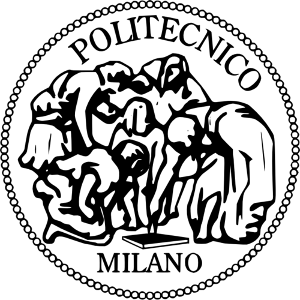
\includegraphics[width=0.20\textwidth]{./pictures/logo_poli}\par
	\vspace{1.5cm}
	{\Large {PowerEnJoy \\ 
		Software Engineering II} \par}
	\vspace{1.5cm}
	{\LARGE \textbf{Requirements Analysis and Specification Document} \par}
	\vspace{1.5cm}
	{\Large\itshape Giovanni Scotti, Marco Trabucchi\par}
	\vspace{2cm}
	\vfill
	% Bottom of the page
	{\large Document version: 2\par}
	{\large \today \par}
\end{titlepage}

%Make the table of contents
\tableofcontents

%INTRODUCTION
\chapter{Introduction}
\label{ch:Introduction}

\section{Purpose}
%purpose
The Design Document is intended to provide a deeper functional description of the \emph{PowerEnJoy} system-to-be by giving technical details and describing the main architectural components as well as their interfaces and their interactions. The relations among the different modules are pointed out using UML standards and other useful diagrams showing the structure of the system.

The document aims to guide the software development team to implement the architecture of the project, by providing a stable reference and a single vision of all parts of the software itself and clearly defining how they work.

\section{Scope}
The product is a digital management system to support a car-sharing service that exclusively employs electric cars.

The system consists of a back-end server application that manages rental requests remotely and three front-end applications:

\begin{itemize}
\item A web-based application to provide the final user with a friendly interface to take advantage of the services of \hbox{\emph{PowerEnJoy}};
\item An application that runs on the existing on-board computers provided on each vehicle, used to interact with the car itself, unlock it and access the GPS/sat-nav service;
\item A mobile application that allows the user to easily access the service anywhere he/she needs to.
\end{itemize}
%serve per modellare i requisiti relativi al sw del computer di bordo [vd specifiche p.3 sez.5]
%"The user is notified of the current charges through a screen on the car"

The system is intended for only one type of user: drivers, who should be allowed to register and access the system via username and password, in order to make the renting and payment processes easier and quicker to carry out. Moreover, the system aids the users by locating nearby available vehicles and keeps track of the distance driven, all while notifying them about the amount of money they are being charged. Predefined safe parking areas are signaled by an on-board computer.

Lastly, the system aims to motivate drivers to maintain a virtuous behavior providing discounts when it detects signs of responsible and ecologic actions.


\section{Goals}
The goals of \hbox{\emph{PowerEnJoy}} are the following:

\begin{enumerate}
\item Let the user register to the service and login via the provided credentials;
\item Let the user manage his/her own profile;
\item Let the driver find the location of nearby available cars and reserve a chosen car;
\item Improve the efficiency of the service by assuring that no car stays reserved for more than an hour if not actually in use;
\item Allow the user to easily access the cars by unlocking them once the driver is in proximity;
\item Automatically manage payments in order to make the service quicker and more dynamic to use; 
\item Allow the user to start a ride, drive to his/her destination and finish the ride with the car he/she reserved;
\item Incentivize responsible behaviors, providing discounts for the worthiest users and additional charges for bad users.
\end{enumerate}

\section{Definitions, Acronyms and Abbreviations}
\begin{description}
\item[RASD:] Requirements Analysis and Specification Document.
\item[System:] The software system-to-be, in all of its entirety.
\item[Driver:] See \textbf{User}.
\item[User:] Any person subscribed to the service who rents a car using \hbox{\emph{PowerEnJoy}}.
\end{description}



\section{References}
This document follows the guidelines provided by ISO/IEC/IEEE 29148:2011~\cite{ieee-29148} and IEEE 830-1998~\cite{ieee-830} respectively related to the requirements engineering for systems and software products and the recommended practice for software requirements specifications.

Moreover it is strictly based on the specifications concerning the RASD assignment~\cite{se-assignments} for the Software Engineering II project, part of the course held by professors Luca Mottola and Elisabetta Di Nitto at the Politecnico di Milano, A.Y. 2016/17.

\section{Overview}
This document consists of three sections:

\begin{description}
\item[Section 1: Introduction.] A general introduction and overview of the system-to-be purpose, scope and goals, along with some important information about this document.
\item[Section 2: Overall description.] It describes the general factors that affects the product and its requirements. The section provides a background for those requirements which are defined in detail in Section 3 and makes them easier to figure out.
\item[Section 3: Specific Requirements.] All the software requirements are specified to a level of detail which is sufficient to let the designers satisfy them. Both functional and non-functional requirements are mentioned.
\end{description}
At the end of the document are an \textbf{Appendix} and a \textbf{Bibliography}, providing additional information about the sections listed above.

\chapter{Overall Description}
\label{ch:Overall_Description}

\section{Product Perspective}
%This should list each system interface and identify the functionality of the software to accomplish the system requirement and the interface description to match the system.
\subsection{User interfaces}
The users have two ways to access the system: a web application can be executed on any personal computer while a mobile application provides flexibility, portability and can be used literally everywhere. Despite the fact that the hardware interfaces running the application are rather different, a unified and common user interface is provided. It should be user friendly and very intuitive to allow everyone to easily use it without any specific knowledge.

Moreover the users have to interact with the on-board computer installed on each electric vehicle, therefore it should offer an interface as straightforward as the one implemented by the web and mobile applications.

%INSERIRE IL REFERENCE A CONSTRAINTS
\subsection{Hardware interfaces}
The web application can be executed on any general purpose computer that complies with the minimum system requirements specified in subsection \ref{ssec:hlimit}.

The mobile application has to exchange data with the GPS module located on any recent smart-phone. Moreover it has to access the mobile broadband in order to communicate with the main system server.

An on-board computer is set up in each electric car and it talks to the vehicle control unit through the CAN bus and to the system server via the mobile broadband.

\subsection{Software interfaces}
The web based application must support the main browsers such as IE, Google Chrome and Mozilla Firefox. The mobile application has to be compatible with iOS and Android. The server side of the application, that is the system back-end, stores data in a relational DBMS and runs on any web server that supports Java.
%DA RIVEDERE
The back-end has mainly to deal with:
\begin{itemize}
\item car reservation
\item payments
\item data storage and management
\item customer account maintenance
\end{itemize}

\section{Product Functions}
The system allows users to reserve available cars, to manage their requests and charge them for the rental.

The users can:
\begin{itemize}
\item Register to the service;
\item Login with their personal account;
\item Edit and manage personal information;
\item Delete their existing account;
\item Locate nearby available-to-rent vehicles;
\item Reserve one of said cars for a fixed amount of time;
\item Unlock the reserved vehicle based on their mobile device GPS position;
\item Alternatively, unlock the reserved car by inserting a vehicle-specific code (found on the windshield) into the application;
\item Start the engine by inserting their PIN;
%solo cose che può fare o anche informazioni che può ricevere? notifica parcheggi e spesa corrente
\item Perform payments for the used service via credit card or \emph{PayPal\textsuperscript{TM}}.
\end{itemize}

\section{User Characteristics}
Target of the service are \emph{drivers} that wish to rent a car.

The base assumption is that every registered user is in possess of a driving license which is valid in the country where he/she makes use of the service.

Moreover, the user must have the means of accessing the service from anywhere: this includes having the possibility to use a stable internet connection both from a mobile device and a stationary one such as a laptop or desktop PC.

Lastly, the user should provide the system a valid payment method upon the act of registration to the service.

\section{Constraints}
\subsection{Regulatory policies}
The system must be allowed by the user to collect, process and store personal data. Furthermore the system is capable to delete all the personal data on user request and to keep track of each payment.

The user has the responsibility to use the system properly in order to comply with the local laws and policies.

\subsection{Hardware limitations}
The system should met the following limitations:
\begin{itemize}
\item Mobile application:
	\begin{itemize}
	\item[>] 3G UMTS connection at its maximum speed of 2 Mb/s
	\item[>] 50 MB of available space
	\item[>] 1 GB of RAM
	\item[>] GPS module
	\end{itemize}
\item Web application:
	\begin{itemize}
	\item[>] Internet connection at 7 Mb/s
	\item[>] 800x600 screen resolution
	\end{itemize}
\end{itemize}

\subsection{Parallel operation}
The system must support parallel operations from different users and the DBMS relies heavily on concurrent transactions.

\subsection{Reliability requirements}
The system reliability, that is the probability to operate without a failure for a specific period of time, must be 99\%.

\subsection{Criticality of the application}
Life-critical applications do not concern the system to be developed.

\section{Assumptions and Dependencies}
For the rest of the RASD, the following assumptions are given for granted:

\begin{itemize}
\item The GPS location of users and cars is always functioning and accurate, with an uncertainty of $\pm$1 m; 
\item All users can access a reliable and stable internet connection;
\item The users' mobile devices feature a working GPS;
\item All users are always charged the correct amount after the ride;
\item The on-board computers always notify the correct charge to the driver during the ride;
\item All cars unlock properly upon insertion of the code by the user who reserved them or in case he/she is detected to be in proximity;
\item The equipment of the cars always gives a correct reading of the number of passengers, driver included, for the current ride;
\item The number of passengers never changes for the duration of the ride;
\item Whenever a car is left with more than 80\% of the battery empty, it is refueled before becoming available again;
\item If a user reserves and uses a car he/she is the one who drives it and is responsible for the associated trip;
\end{itemize}

\section{Future Extensions}
The system implementation will open the possibility of including new features. For example:

\begin{itemize}
\item The possibility of including more categories of vehicles, such as motorcycles and bycicles;
\item The possibility of receiving active feedback from the users, mainly concerning car conditions;
\item The possibility for everyone, registered and unregistered people, of notifying \emph{PowerEnJoy} of incorrect or unsafe situations involving their vehicles.
\end{itemize}

\chapter{Specific Requirements}
\label{ch:Specific_Requirements}

\section{External Interface Requirements}
\subsection{User interface}
The user interfaces must be strongly user-friendly, in order to provide an easy and intuitive way to access the system. The following constraints have to be satisfied by the web and mobile applications:
\begin{itemize}
\item The first page must always ask the user to login or register to the service;
\item The main page must show a map with a marker for all the locations of all nearby available cars inside the Safe Area;
\item The interface must offer the possibility to choose between a set of different languages;
\item A toolbar must be visible in every screen except the first page;
\item The toolbar must offer a quick and simple overview of the main system functionalities (reserve a car, reservations history, modify personal information...);
\item The user interface must dynamically adapt to the screen size;
\item In order to simplify the user experience, the web application and the mobile one must use the same graphical elements and layouts.
\end{itemize}
With respect to the on-board computer application, the restrictions are the following:
\begin{itemize}
\item After the car has been unlocked, the display of the on-board computer must turn on and show a screen thats allows the user to input his/her PIN in order to start the ride;
\item Once the ride starts, the screen must clearly show the current charges;
\item Similarly, during the ride, the screen must clearly show the nearby charging spots and visually signal the Safe Area boundaries;
\item When the car is available, the screen must always be off.
\end{itemize}
Some mock-ups that give an overall idea of the interface structure of the applications are provided in the next section (\ref{fun_req}).
In addition to that several application-dependent constraints are provided:
\begin{itemize}
\item Web application
	\begin{itemize}
	\item[] All the web pages must abide by the W3C standards to ensure a long-term growth of the application and take the full advantage of HTML5 markup language and CSS.
	\end{itemize}
\item Mobile application
	\begin{itemize}
	\item[] Both the Android and iOS versions must follow the design guidelines provided by the respective platform manufacturers.
	\end{itemize}
\item Server application
	\begin{itemize}
	\item[] The server application must be easily configurable via a XML file and use the APIs provided by the payment handler to interface with its information system.
	\end{itemize}
\item On-board computers application
	\begin{itemize}
	\item[] The application mounted on on-board computers must use the APIs provided by the vehicle manufacturer to interface with the cars.
	\end{itemize}
\end{itemize}

\subsection{Hardware interface}
The most relevant aspect to highlight, in addition to section \ref{hw_int}, is the ability of the system-to-be to communicate with the car systems via the embedded computer located in the car itself that takes the advantage of the on-board computer application to be developed. The on-board computer can communicate with the mobile broadband thanks to a SIM and provides a GPS module exploitable by the car-side of the application.

\subsection{Software interface}
The server side of the application, that represents the back-end of the system-to-be, requires the following software products:
\begin{itemize}
\item Java SE 8 - \url{http://www.oracle.com/technetwork/java/javase/overview/index.html}
% Java SE? Non EE? Forse più tardi lo modifichiamo...
\item MySQL 5.7 - \url{http://dev.mysql.com/}
\end{itemize}

The embedded on-board computer located in each car provides a Linux OS that is capable to run C/C++ programs. Moreover the car-side of the application can use specific software libraries provided by the manufacturer to access the car systems the computer is connected with.

\subsection{Communication interface}
The clients communicate with the server via HTTPS protocol by using TCP and default port 443.
Moreover a safe and stable connection is also established between the server and the payment handler whenever the user performs a payment.

\section{Functional Requirements} \label{fun_req}
\subsection{Register}
\subsubsection{Purpose}
The user who wants to subscribe to the \emph{PowerEnJoy} service can carry out the registration process through the mobile application or the web one. First of all the user has to fill a registration form with his/her personal information and accept the Terms and Conditions agreement otherwise the procedure will be aborted.

As soon as the user submits the data, the system checks all the information and sends a confirmation e-mail to the specified e-mail address including the password to access the service and the personal PIN required to start the car engine.

\subsubsection{Scenario 1}
Marta would like to register to the \emph{PowerEnJoy} rental service from her computer. She opens the browser and loads the registration page by clicking on the "sign up" button located in the \emph{PowerEnJoy} login page. She fills in the registration form and agrees the service Terms and Conditions. Then Marta submits everything to the system, that checks the personal data. Personal PIN and password are sent to Marta in a confirmation e-mail notifying the successful registration.

\subsubsection{Scenario 2}
Yuri cannot afford a car and therefore decides to take advantage of the \emph{PowerEnJoy} service. He accesses the login page from his mobile phone and taps the "sign up" button since he is not a registered user. Then he fills in the form and accepts the Terms and Conditions.

Unfortunately he forgets to fill in his own tax code and the system does not allow him to carry out a successful registration notifying the forgetfulness. Afterwards Yuri completes the procedure by filling the whole form. The system communicates the successful registration and sends him a confirmation e-mail containing PIN and password.

\subsubsection{Use-case}

The use-case of the registration procedure is analyzed in Table \ref{register_uc}.

\subsubsection{Activity diagram}

The activity diagram of the registration procedure is shown in Figure \ref{register_act}.

\subsubsection{Functional requirements}
\begin{enumerate}
\item The user must not enter an already registered e-mail address to perform the registration process;
\item The user must provide the following personal information:
	\begin{itemize}
	\item e-mail address
	\item name
	\item surname
	\item ID card number
	\item tax code
	\item license ID number
	\item address
	\item phone number
	\item credit/prepaid card or \emph{PayPal\textsuperscript{TM}} account credentials
	\end{itemize}
\item There must not be another subscribed user with the same identity card number, tax code or license ID;
\item If the user does not agree the service Terms and Conditions, the registration process is canceled;
\item The system must send an e-mail containing PIN and password to the e-mail address specified by the user when he/she clicks on "Submit" button and all the required information has been entered;
\item The system allows the user to exit the registration process at any time;
\item The system must allow the user to provide either a valid credit/prepaid card number or \emph{PayPal\textsuperscript{TM}} account credentials to perform the payments;
\item The PIN provided by the system in the confirmation e-mail is made by only digits and has a length of 6;
\item The password provided by the system in the confirmation e-mail is made by both digits and letters (capital and not) and has a length of 8.
\end{enumerate}

\begin{table}[H]
\begin{center}
\begin{tabular}{p{0.3\textwidth} | p{0.7\textwidth}}
\hline
Actor & User\\
\hline
Goal & Goal 1\\
\hline
Input Condition & The user wants to subscribe to the service.\\
\hline
Event Flow & 
\begin{enumerate}
\item The user opens the \emph{PowerEnJoy} home page or the mobile application and clicks or taps on the "Sign up" button;
\item The registration form is loaded and the user fills in all the fields with his/her personal information;
\item The user agrees the service Terms and Conditions by checking the corresponding box;
\item The user clicks on "Submit" button;
\item The system saves the data in its database and sends a confirmation e-mail containing PIN and password to the new registered user.
\end{enumerate} \\
\hline
Output Condition & The system tells the user he/she is successfully subscribed and lets him/her to log in with the provided credentials.\\
\hline
Exception & When some exceptions occur, the system reloads the registration form and goes back to step 2 of Event Flow notifying the user about the error. This happens when the following requirements are not satisfied: 1, 2, 3.

The registration process is aborted when the user decides not to carry it out completely or when requirement 4 generate an exception.\\
\hline
\end{tabular}
\end{center}
\caption{Register use-case}
\label{register_uc}
\end{table}

\begin{figure}[H]
\begin{center}
		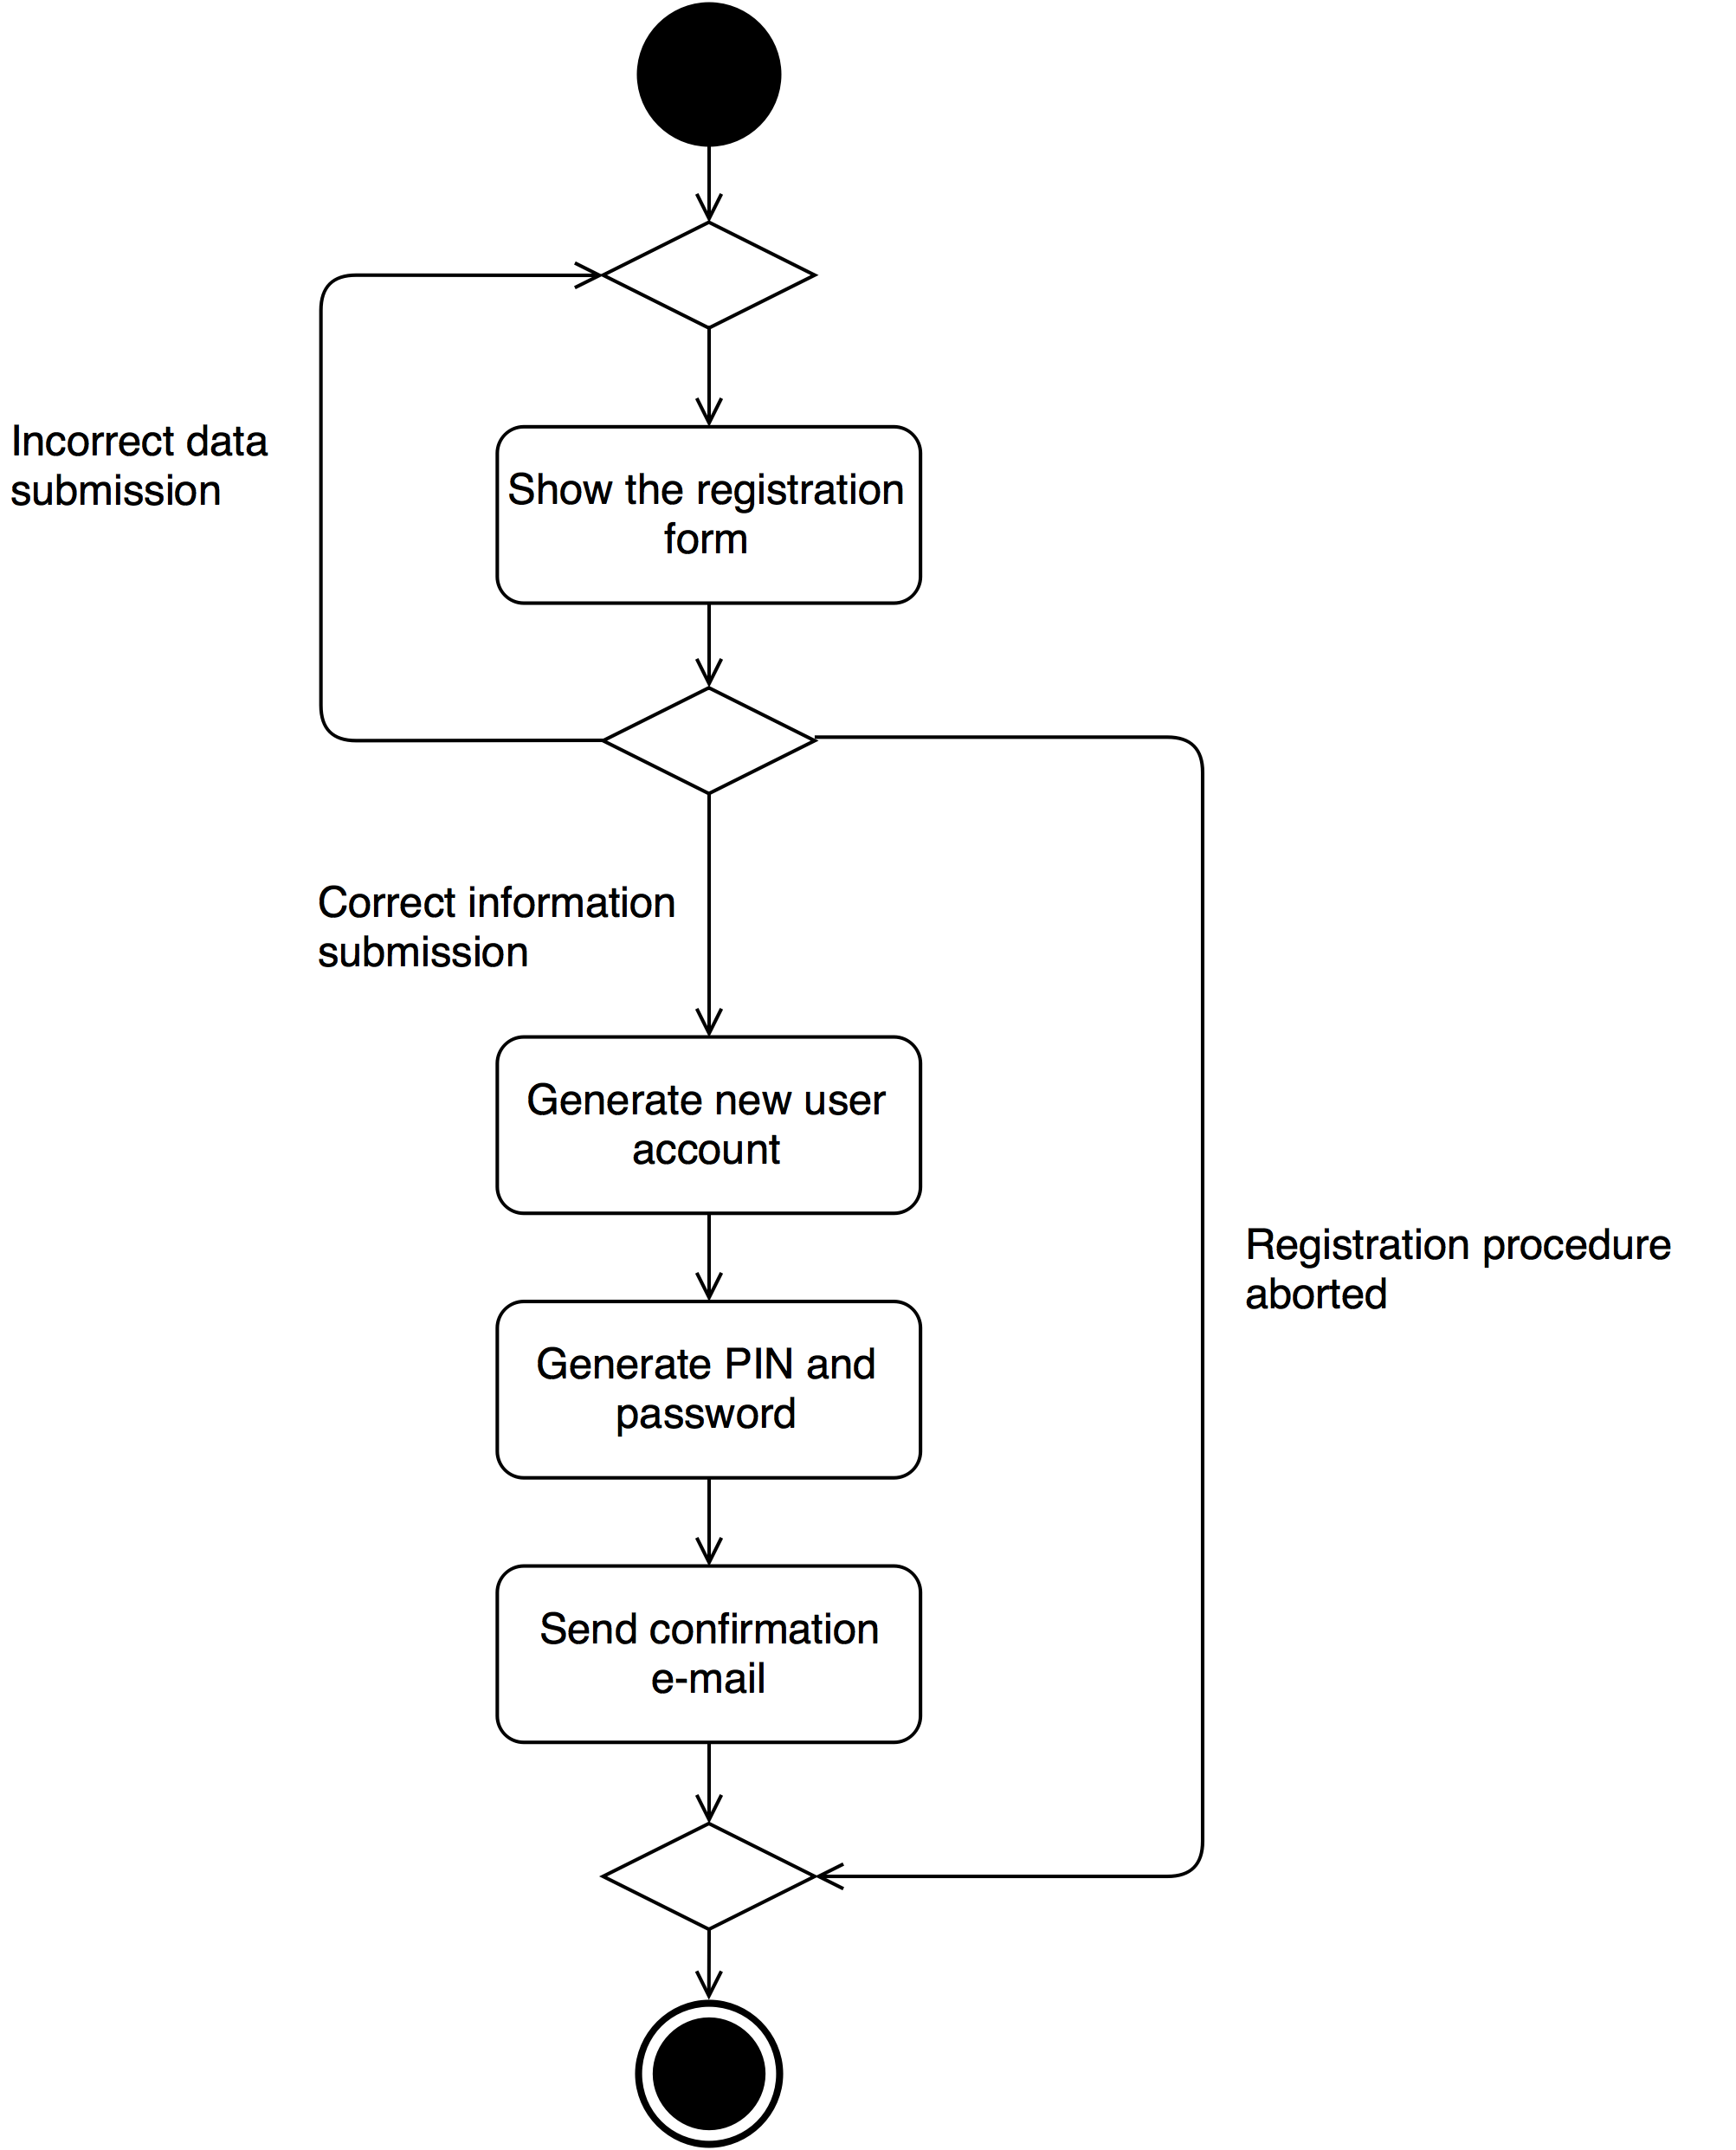
\includegraphics[width=\textwidth]{./specific_requirements/features/diagrams/registration_activity.png}
		\caption{Activity diagram of the registration process from the system point of view}
		\label{register_act}
\end{center}
\end{figure}

\begin{figure}[H]
\begin{center}
		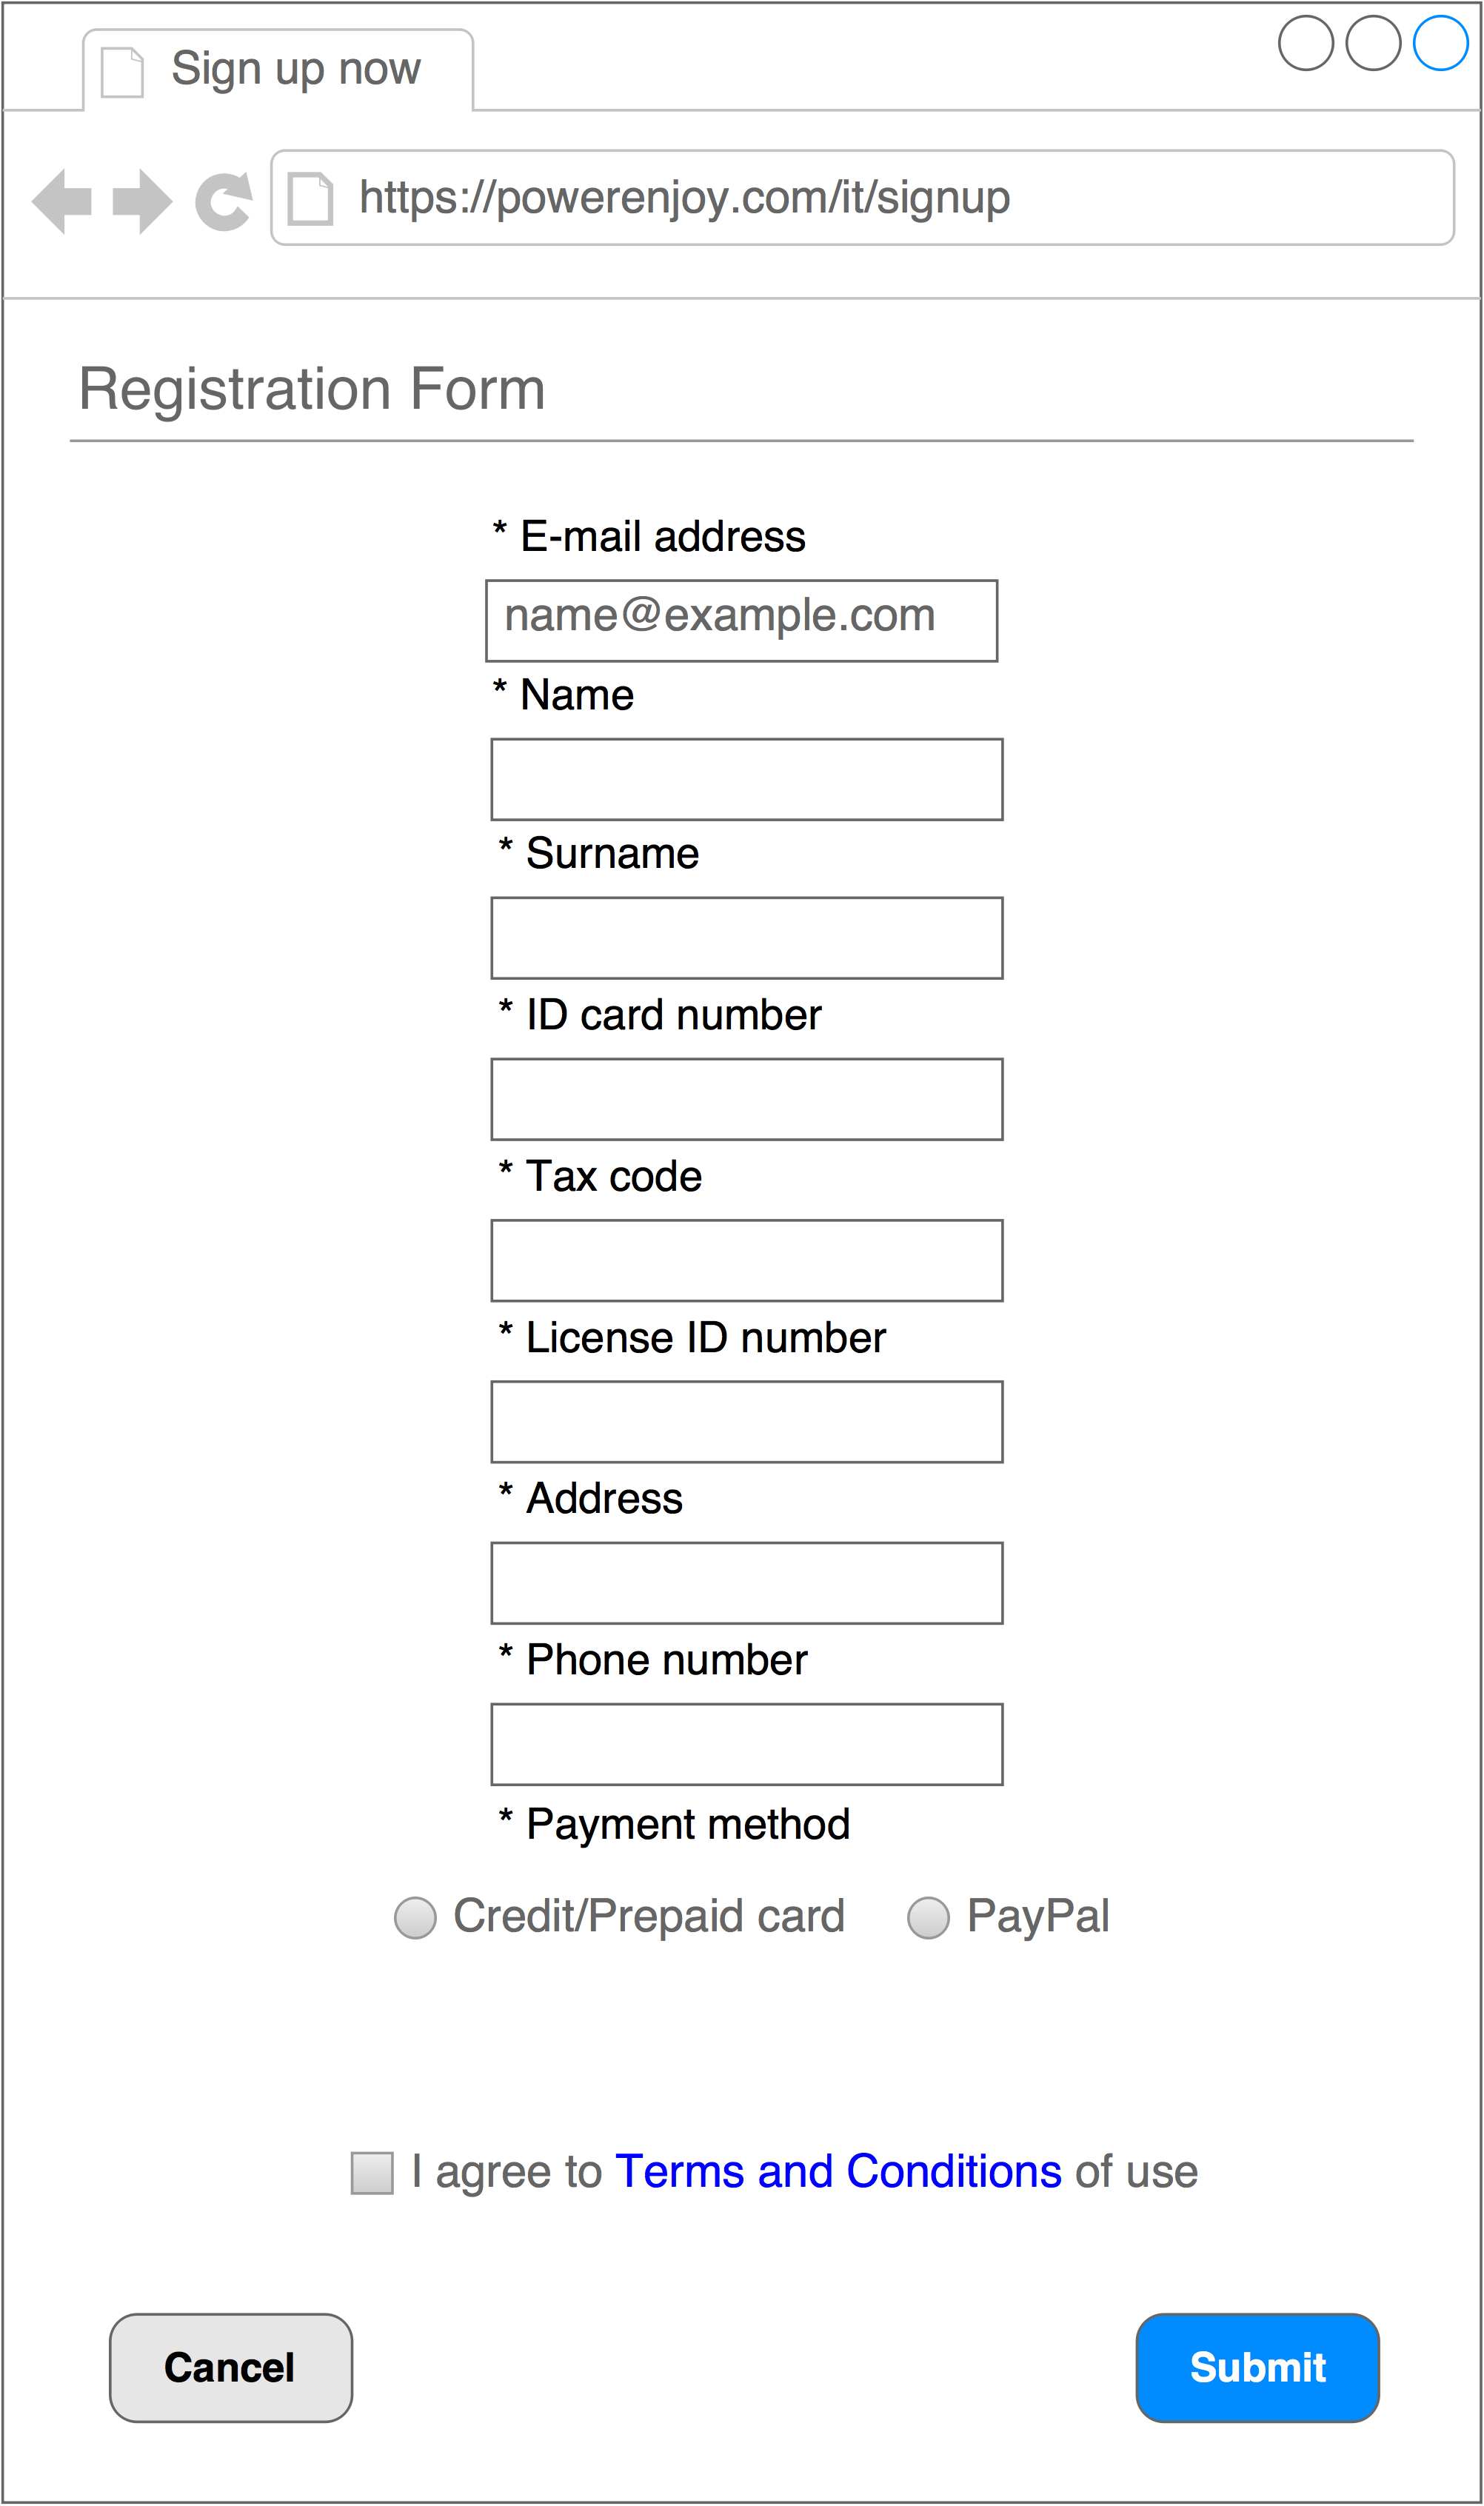
\includegraphics[width=0.8\textwidth]{./specific_requirements/features/diagrams/web_registration.png}
		\caption{Concept of the sign up webpage}
\end{center}
\end{figure}

\subsection{Login}
\subsubsection{Purpose}
The main purpose of the login feature is to grant the access of the \emph{PowerEnJoy} service to any registered user. The system requires a valid e-mail address and password to login without generating any error.

In addition to that, the login screen offers the chance to recover a forgotten password. The user clicks on "forgot password?", a new one is sent to his e-mail address immediately and he/she can carry out the login procedure with the new password provided by the system.

\subsubsection{Scenario 1}
Mike would like to rent a car for having a ride in a beautiful sunny day. In order to do that he needs to access the system by means of his credentials. He opens the \emph{PowerEnJoy} home page and enters his e-mail address and his password. Then Mike clicks on "login" and, due to the fact that everything is correct, he obtains the access as a logged user.

\subsubsection{Scenario 2}
Bill wants to take the advantage of the \emph{PowerEnJoy} service. He opens the home page and he is asked for his e-mail address and password. He is aware of his e-mail address, but he does not remember the password. After some time spent trying to recall his personal password, Bill inputs his e-mail address and decides to click on "forgot password?". Right away the system sends a new password to the specified e-mail address. Bill can now enter the system using the new password.

\subsubsection{Use-case}

\begin{table}[H]
\begin{center}
\begin{tabular}{p{0.3\textwidth} | p{0.7\textwidth}}
\hline
Actor & User\\
\hline
Goal & Goal 1\\
\hline
Input Condition & The user is already registered to the system and wants to login.\\
\hline
Event Flow & 
\begin{enumerate}
\item The user opens the \emph{PowerEnJoy} home page or the mobile application and the system shows the login page;
\item The user enters his/her e-mail address and password.
\end{enumerate} \\
\hline
Output Condition & The system lets the user to log in if the provided credentials are valid and loads his/her personal home page.\\
\hline
Exception & 
If the e-mail address provided by the user has never been registered to the system or if the password does not correspond to the entered e-mail, the system notifies the user with an error message. If the user enters wrong credentials three times in a row, the system will prevent any attempt for the following 30 seconds.\\
\hline
\end{tabular}
\end{center}
\caption{Login use-case}
\label{login_uc}
\end{table}

\subsubsection{Statechart diagram}

\begin{figure}[H]
	\centering
		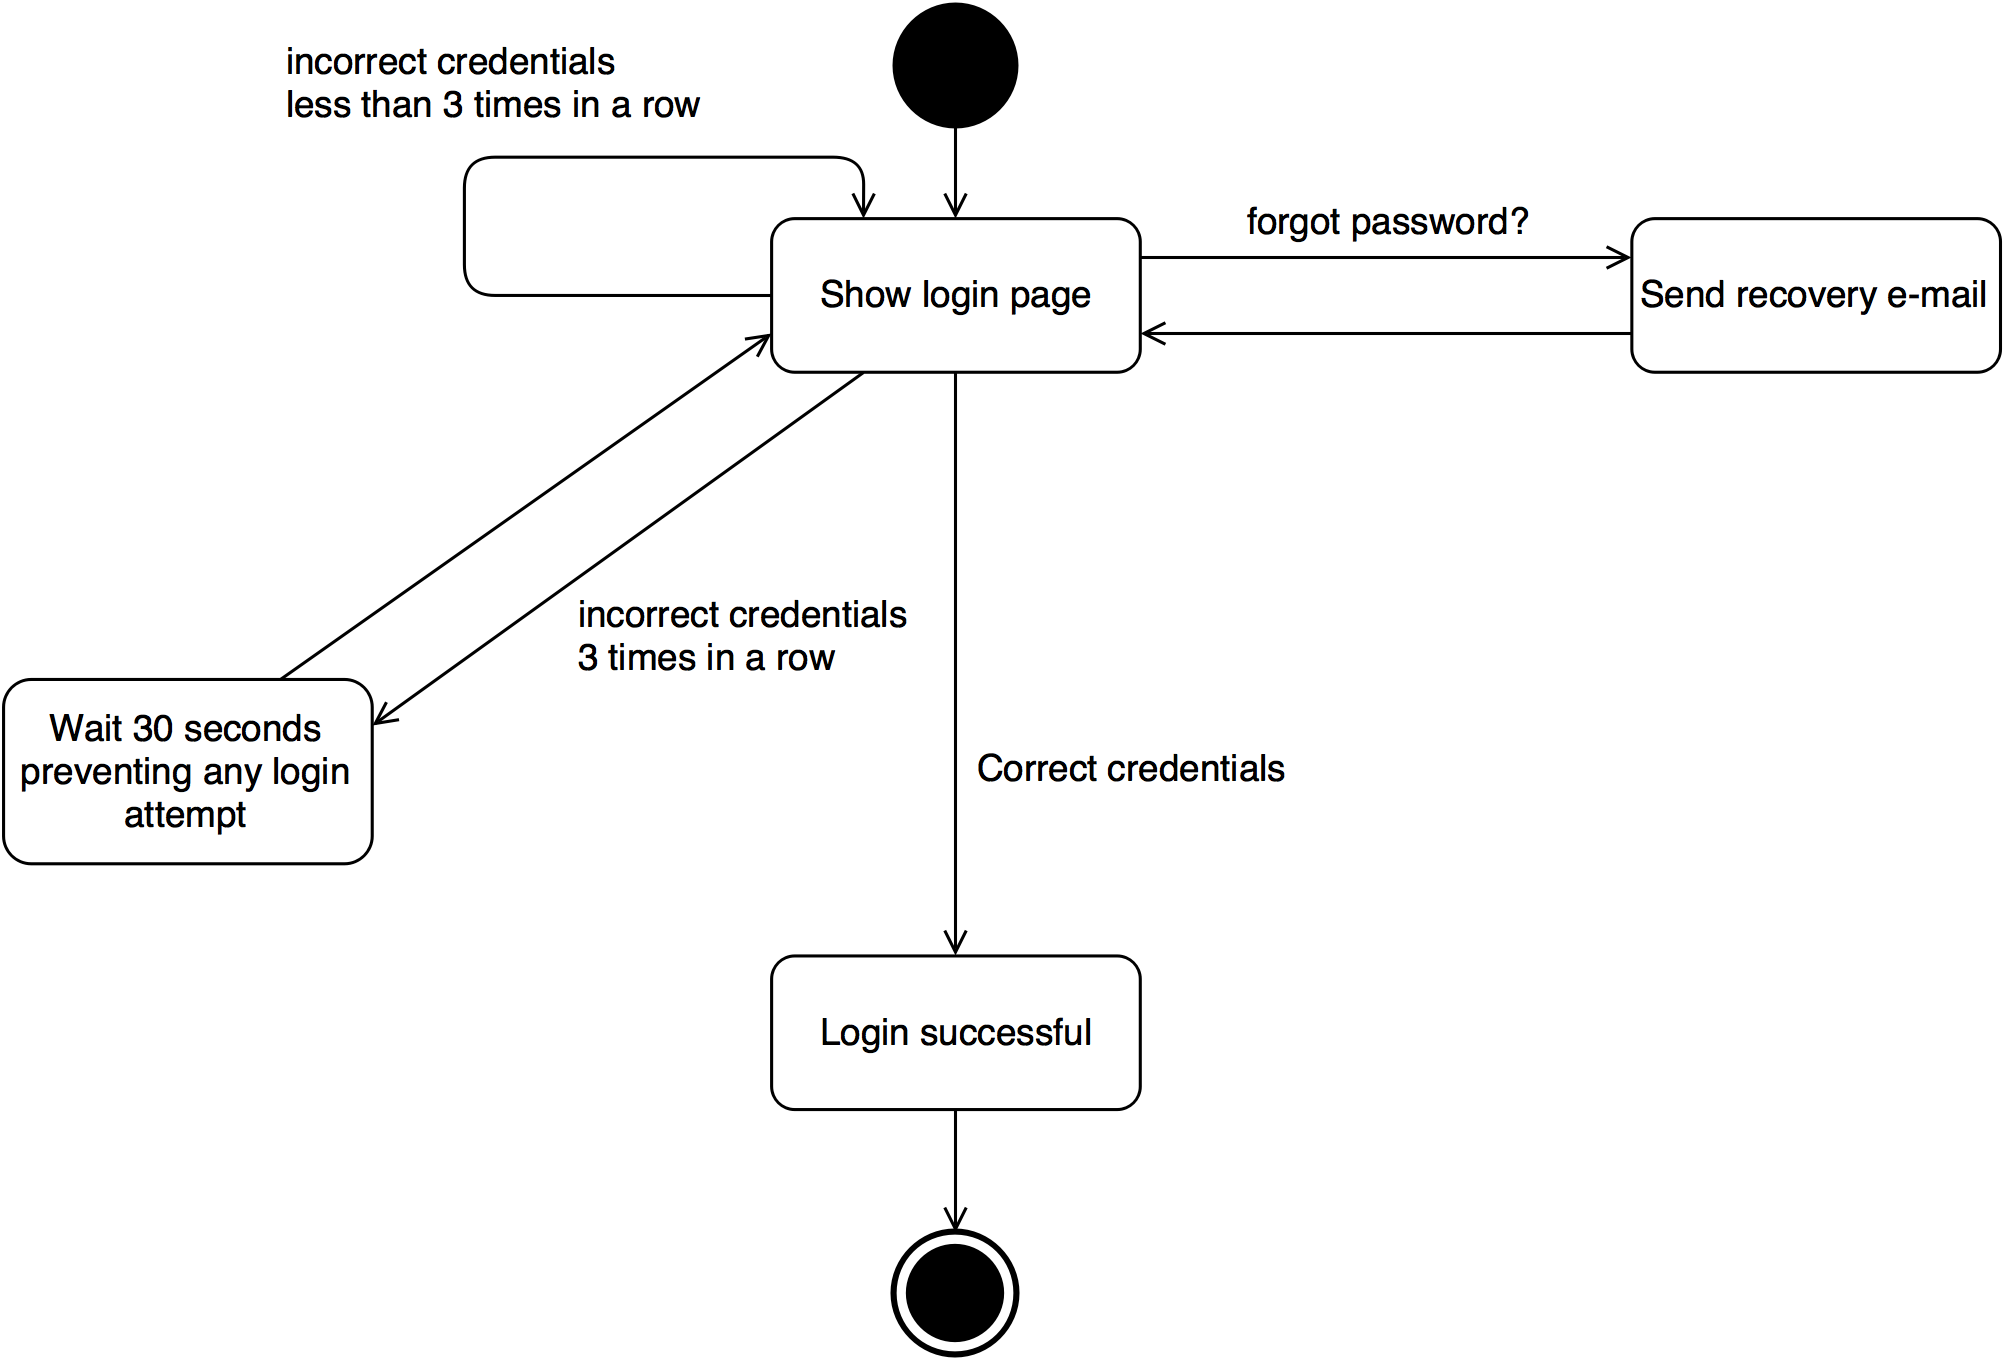
\includegraphics[width=\textwidth]{./specific_requirements/features/diagrams/login_statechart.png}
		\caption{Statechart of the login process from the server application point of view}
\end{figure}

\subsubsection{Functional requirements}
\begin{enumerate}
\item The user must be already registered to the system in order to perform a successful login;
\item The user must be aware of his e-mail address and password to successfully obtain the system access;
\item The password provided by the user must correspond to the specified e-mail address;
\item The system sends a new password to the specified e-mail address if and only if the specified e-mail address is valid, registered to the system and the user clicks on "forgot password?";
\item After requesting a new password, the system must allow the user login with the new provided password;
\item After three times the entered password is wrong, the system allows a new attempt 30 seconds later.
\end{enumerate}

\begin{figure}[H]
	\centering
		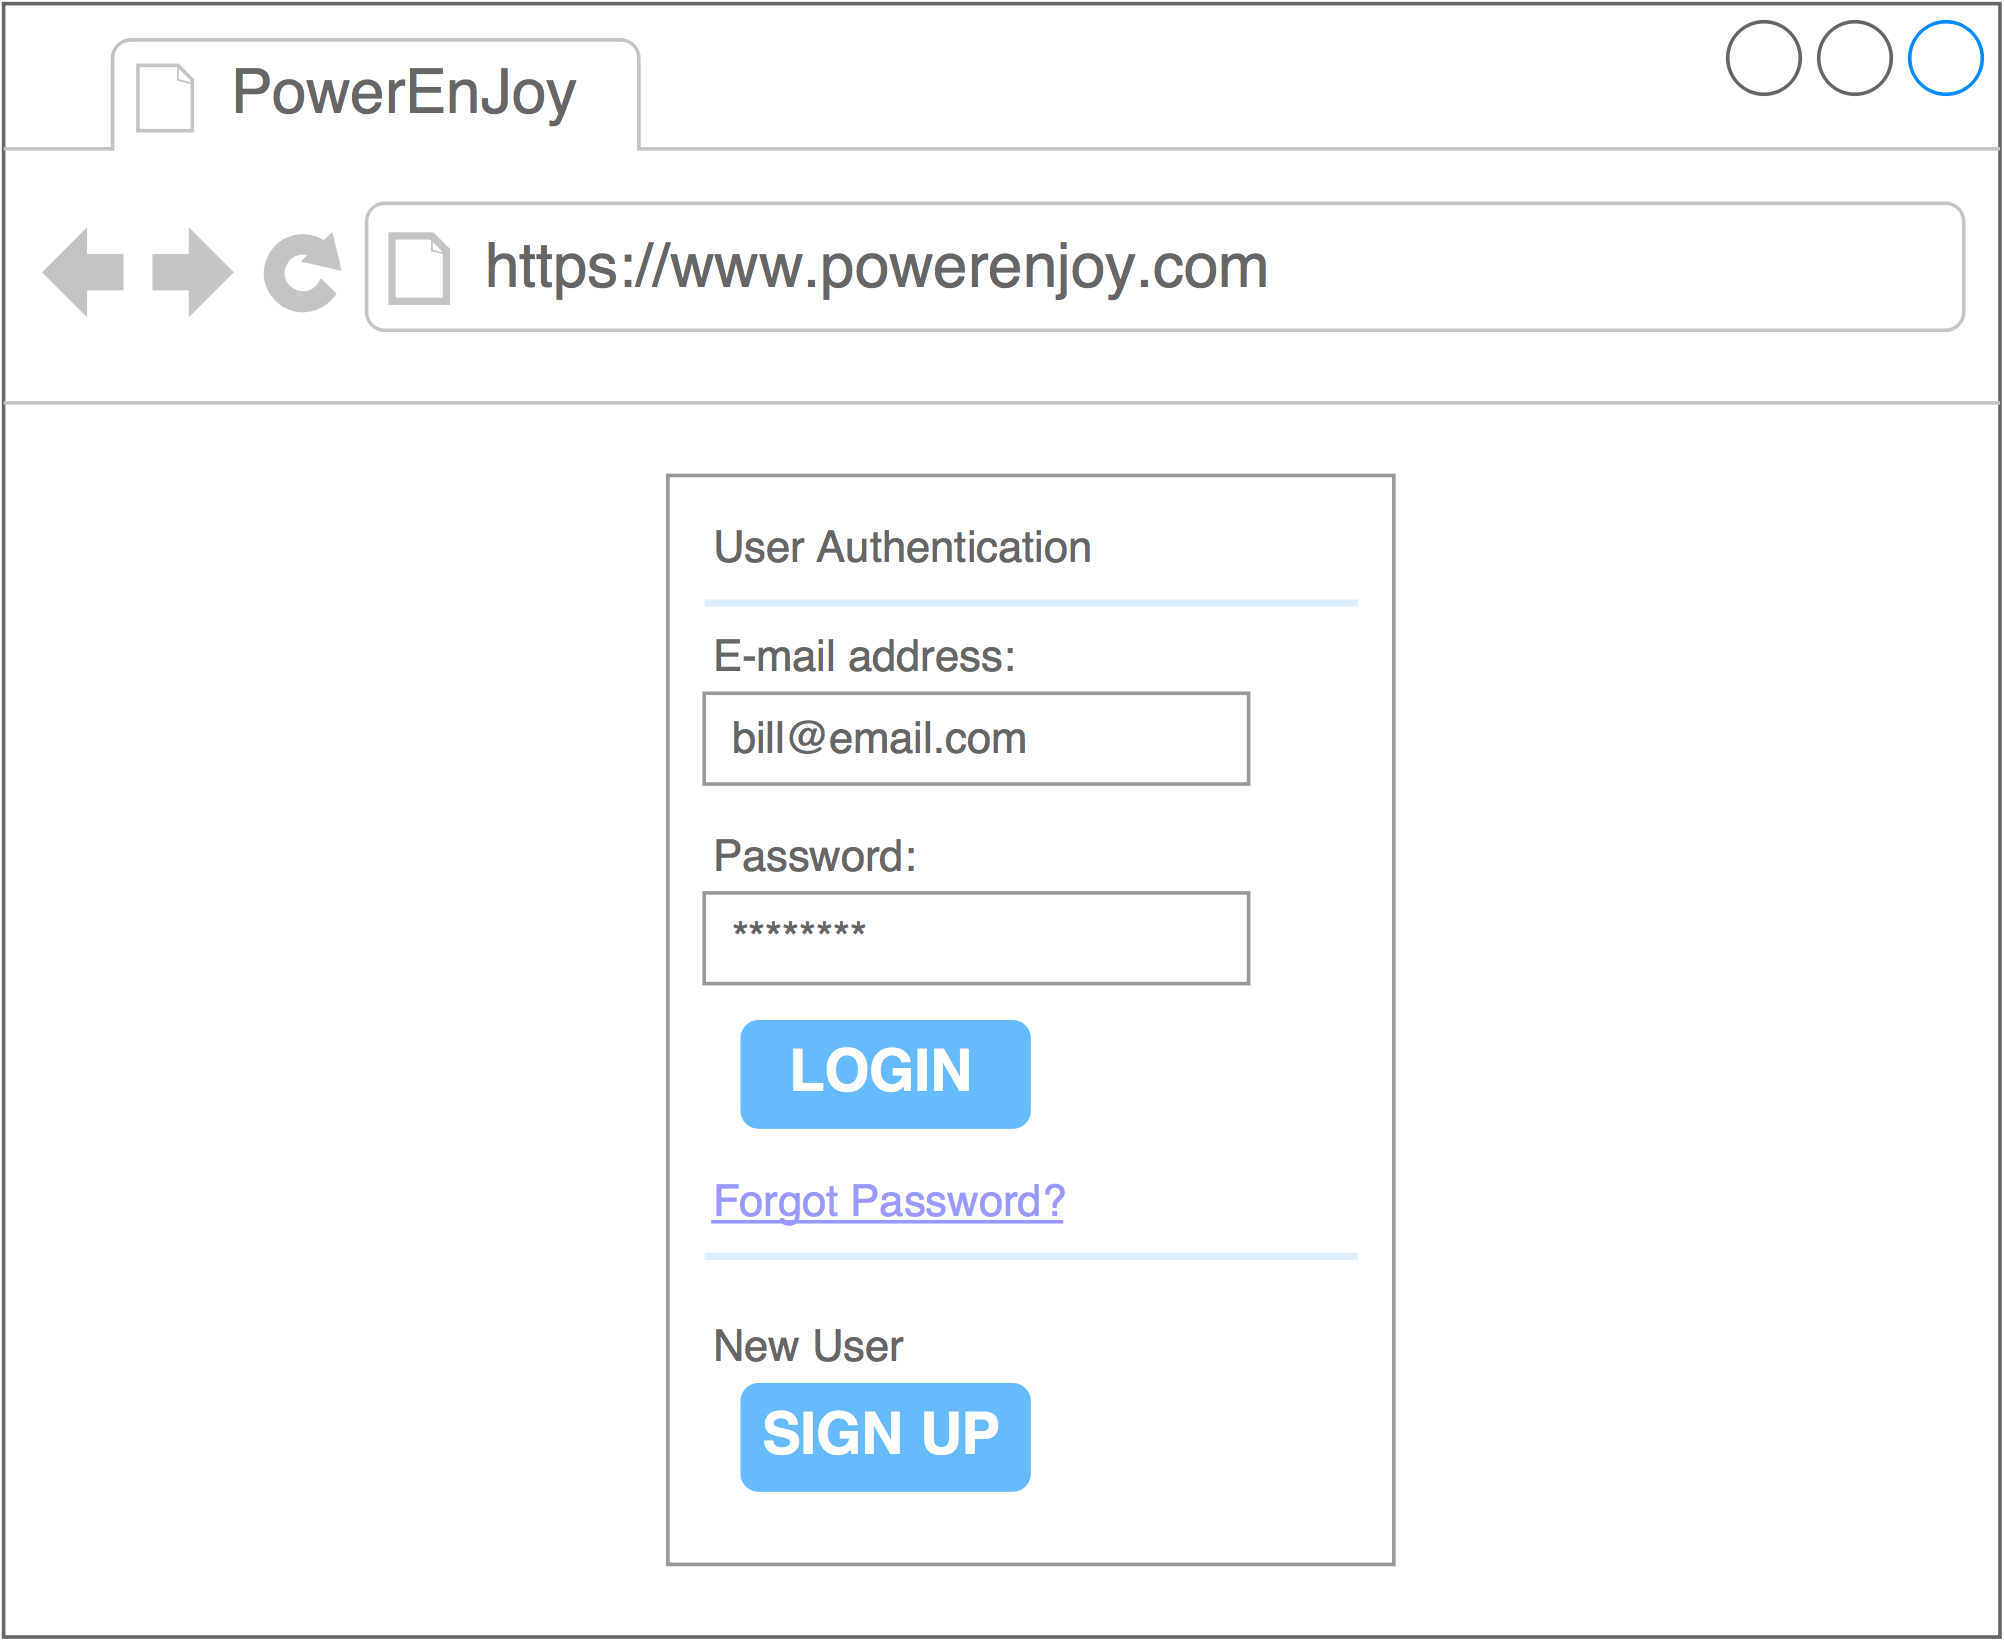
\includegraphics[width=0.8\textwidth]{./specific_requirements/features/diagrams/web_login.png}
		\caption{Concept of the login webpage}
\end{figure}

\begin{figure}[H]
	\centering
		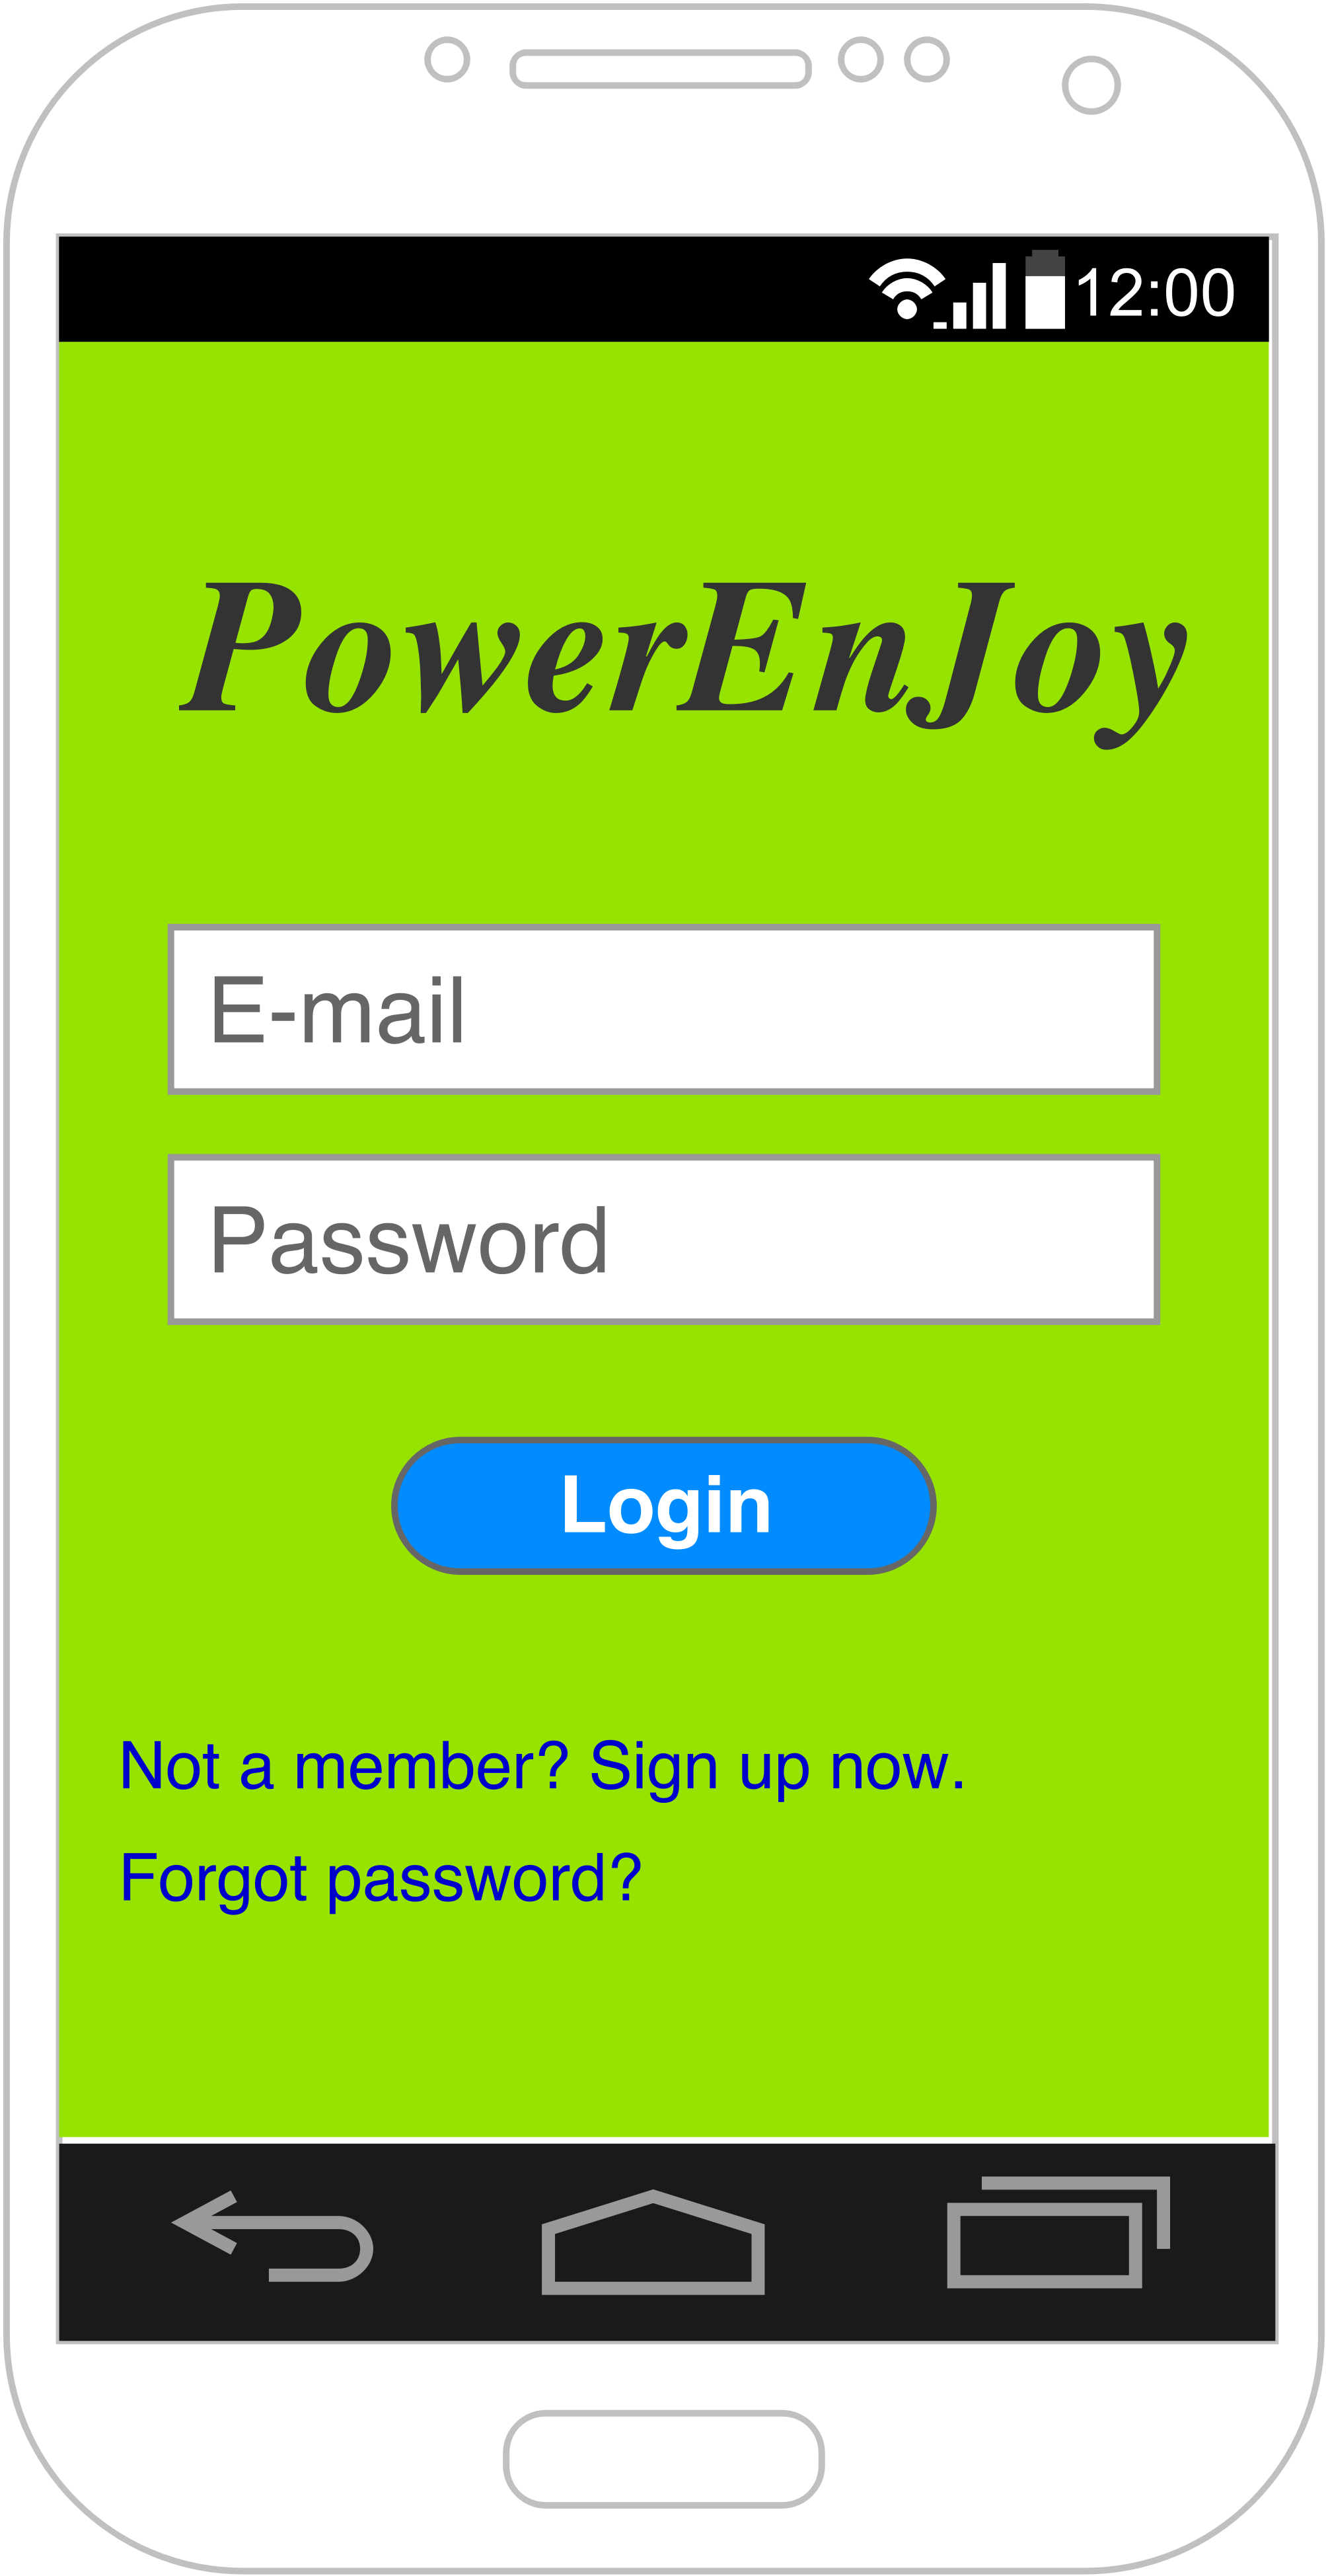
\includegraphics[width=0.4\textwidth]{./specific_requirements/features/diagrams/mobile_login.png}
		\caption{Concept of the mobile version of the login screen}
\end{figure}

\subsection{Manage profile}
\subsubsection{Purpose}
Both the mobile application and the web one provide the chance to any user to view and update the personal profile information. The system is able to provide also information about the reservations and rides history as well as the respective payments.

Moreover the user is allowed to delete his/her account if the service is no longer needed.

\subsubsection{Scenario 1}
Anna has already carried out the registration process, but she does not like the password the system provided her because it is hard to remember. Therefore she decides to log in from her mobile phone and access the personal information area through the designated toolbar.

She taps \emph{"Edit Profile"} and the system allows her to edit profile information. Anna enters the old password in the designated field as well as the new one, that must be entered twice to avoid unwanted errors. Then Anna selects \emph{"Confirm"} and the system notifies her about the successful update.

\subsubsection{Scenario 2}
Flavio has recently renewed his identity card. In order to take the advantage of the \emph{PowerEnJoy} service, he must update his profile information. Flavio opens the browser, reaches the \emph{PowerEnJoy} home page and authenticates himself carrying out the login procedure. 

Then he access his personal information area and clicks \emph{"Edit Profile"}. He fills in the gap corresponding to the ID card number and, as soon as Flavio is ready, he clicks on the \emph{"Confirm"} button and the system confirms the ID card number has been successfully updated.

\subsubsection{Scenario 3}
Emma wants to delete her \emph{PowerEnJoy} account because she does not need the service anymore. She logs in from her mobile phone and enters her personal information area. She selects \emph{"Edit Profile"}, taps \emph{"Delete Account"} and confirms her choice twice. The system removes immediately all Emma's information from the database. From now on she needs a new account in order to access the system again.

\subsubsection{Use-case}
The overall profile management use-case diagram is shown in Figure \ref{man_profile_uc}. \\
The use-case of view profile procedure is analyzed in Table \ref{view_profile_uc}. \\
The use-case of modify profile procedure is analyzed in Table \ref{modify_profile_uc}. \\
The use-case of delete profile procedure is analyzed in Table \ref{delete_profile_uc}.

\subsubsection{Functional requirements}
\begin{enumerate}
\item The system allows the user to view his/her profile. When the user enters his/her personal information area, the system must display:
	\begin{itemize}
	\item all the user's personal information that has been entered during the registration process;
	\item the rides and reservations history;
	\item the payments history.
	\end{itemize}
\item The system allows user to modify his/her personal information as needed:
	\begin{itemize}
	\item the system allows to change any information except e-mail address and authentication method related ones when the user selects \emph{"Edit Profile"};
	\item the system asks the user to enter the old password and two times the new one whenever he/she needs to change it;
	\item the system allows the user to change the password if and only if the old one has been entered correctly;
	\item the system must not allow the user to change the password if the new one has not been entered twice;
	\item the system makes the change permanent as soon as the user clicks the \emph{"Confirm"} button;
	\item the system allows the user to abort the profile editing at any time.
	\end{itemize}
\item The system allows the user to delete his/her account:
	\begin{itemize}
	\item the system asks for a confirmation twice whenever the user wants to delete his/her account;
	\item the system completely destroys the user's personal information and removes his/her account from the database.
	\end{itemize}
\end{enumerate}

\begin{figure}[H]
\begin{center}
		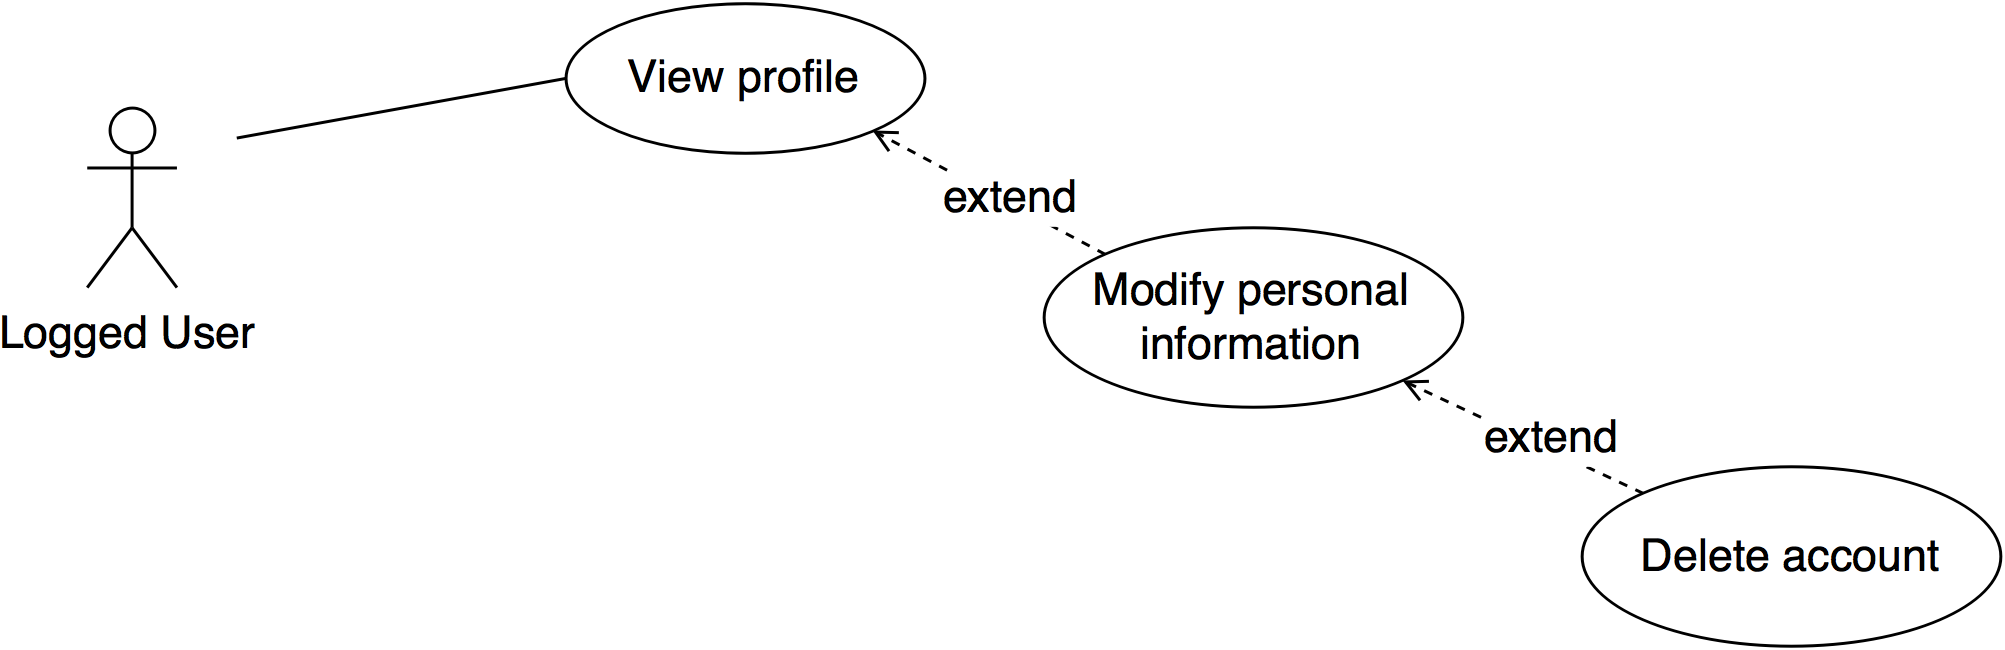
\includegraphics[width=\textwidth]{./specific_requirements/features/diagrams/man_profile_uc.png}
		\caption{Profile management use-case diagram.}
		\label{man_profile_uc}
\end{center}
\end{figure}

\begin{table}[H]
\begin{center}
\begin{tabular}{p{0.3\textwidth} | p{0.7\textwidth}}
\hline
Actor & User\\
\hline
Goal & Goal 2\\
\hline
Input Condition & The authenticated user wants his/her profile information to be displayed.\\
\hline
Event Flow & 
\begin{enumerate}
\item The user enters his/her personal information area.
\item The system loads the page.
\end{enumerate} \\
\hline
Output Condition & The system lets the user check his/her profile, the reservations and rides history as well as the completed payments.\\
\hline
Exception & 
None.\\
\hline
\end{tabular}
\end{center}
\caption{Profile visualization use-case.}
\label{view_profile_uc}
\end{table}

\begin{table}[H]
\begin{center}
\begin{tabular}{p{0.3\textwidth} | p{0.7\textwidth}}
\hline
Actor & User\\
\hline
Goal & Goal 2\\
\hline
Input Condition & The authenticated user wants to edit his/her profile information.\\
\hline
Event Flow & 
\begin{enumerate}
\item The user enters his/her personal information area;
\item The user selects \emph{"Edit Profile"};
\item The system loads the \emph{"Edit Profile"} page;
\item The user enters the new information;
\item The user confirms the desired changes.
\end{enumerate} \\
\hline
Output Condition & The system updates the user's personal information.\\
\hline
Exception & Every time the user does not satisfy one of the requirements listed as number 2, the system simply ignores the modification and reloads the \emph{"Edit Profile"} page.\\
\hline
\end{tabular}
\end{center}
\caption{Modify profile use-case.}
\label{modify_profile_uc}
\end{table}

\begin{table}[H]
\begin{center}
\begin{tabular}{p{0.3\textwidth} | p{0.7\textwidth}}
\hline
Actor & User\\
\hline
Goal & Goal 2\\
\hline
Input Condition & The authenticated user wants to delete completely his/her profile.\\
\hline
Event Flow & 
\begin{enumerate}
\item The user enters his/her personal information area;
\item The user selects \emph{"Edit Profile"};
\item The system loads the \emph{"Edit Profile"} page;
\item The user selects \emph{"Delete Account"};
\item The system asks to confirm and the user confirms;
\item The system asks again to confirm and the user agrees;
\end{enumerate} \\
\hline
Output Condition & The system deletes the user's account.\\
\hline
Exception & If the user decides not to confirm twice, the deletion process is aborted and the \emph{"Edit Profile"} page is reloaded.\\
\hline
\end{tabular}
\end{center}
\caption{Delete profile use-case.}
\label{delete_profile_uc}
\end{table}

\subsection{Reserve Car}
\subsubsection{Purpose}
The reserve car feature is a key service of \emph{PowerEnJoy}. Its main purpose is that of allowing users to choose a nearby car from the ones marked as available on the map, hence signaling their intention of reserving it for an hour. The service can be accessed from the home page of both the web and mobile applications, clicking on the corresponding icon on the toolbar.

The reservation screen shows the user only available cars, based on the information provided by the server. The user can either search for an available car using the mobile application - that is, based on its GPS position - or using the web application, indicating an address around which he wishes to search for a vehicle.

Only one car should be rented at a time, so the system will prevent the user from trying to reserve several cars simultaneously.

\subsubsection{Scenario 1}
Alice is logged in to the \emph{PowerEnJoy} service with her laptop, because she wants to find a car to go meet a friend downtown. To do so, she clicks on the reservation icon and opens the city map. She inputs her address, to indicate that she wants a car not far from her house. The system proceeds to mark the vehicles within the desired location. Alice finds a car that she thinks is reasonably close and clicks on it. The system prompts her asking: \emph{"Do you want to reserve this car?"}. She clicks on the \emph{"Yes"} button, hence forwarding the request of the specific car to the system.

\subsubsection{Scenario 2}
Bob is in town and has just finished shopping. He wants to go back home, but does not want to catch a crowded subway train during the rush hour. For this reason he has logged in to the \emph{PowerEnJoy} application and taps on the reservation icon. The system opens a map that shows the GPS position - provided by Bob's smartphone - and several icons marking nearby available cars. He chooses a vehicle just around the corner and properly confirms his intention of reserving the car for some time; by doing so, his request is forwarded to the server. A few minutes later, he meets a friend that offers him a ride, and decides to accept. So, he logs in to his account again and opens the reservation function. He taps on the \emph{"Release Reservation"} button and the system processes his request by marking the car as available again.

\subsubsection{Scenario 3}
Carla is in need of a car after work, and decides to use a \emph{PowerEnJoy} one. She is looking at the reservation screen and decides to reserve a vehicle by selecting it. Since she is not sure that she will be able to reach the vehicle easily, she tries to reserve a second one after a few minutes. At that point, the system shows her the error message: \emph{"You can only reserve one vehicle at a time. Release your current reservation if you wish to rent this car."}. So she is redirected to the home page again, and the system does not process her second request.

\subsubsection{Use-case}
A more detailed use-case diagram is provided in order to model the possibility of releasing an existing reservation. The detail of the use-case diagram is shown in Figure \ref{request_car_uc}.

The use-case for the standard procedure needed to request a car is analyzed in Table \ref{reserve_car_uc}.
The use-case for the procedure needed to release an existing reservation is analyzed in Table \ref{reserve_car_uc_alt}

\subsubsection{Sequence diagram}
The diagram for the standard behavior of the system in case of a car reservation is shown in Figure \ref{reserve_car_sd}.

\subsubsection{Functional Requirements}
\begin{enumerate}
\item The system must not accept as a valid address one outside the Safe Area, either if it is esplicitly requested by the user or if it is detected by the GPS position;
\item The system must provide the position of all nearby vehicles in a radius of 2 km precisely for every address that was considered valid;
\item The system must mark as available only cars that are not already reserved or out-of-service;
\item If a user tries to reserve a car, but that car has been reserved by another user during the visualization of the available vehicles, the system must notify it with an error message;
\item The system must allow to reserve cars only users that do not have an active reservation, that is to say a reservation not older than an hour;
\item If a user has an active reservation, the system must show as first screen - upon the selection of the reservation function - the recap of said active reservation, including time of expiration and car location;
\item If a user has an active reservation, the system must allow him/her to renounce to it by clicking on the \emph{"Release reservation"} button and confirming his/her intentions;
\item The system must always notify the user of a successful reservation/recess from a reservation, immediately after the action is saved in memory by the server.
\end{enumerate}

\begin{figure}[H]
\begin{center}
		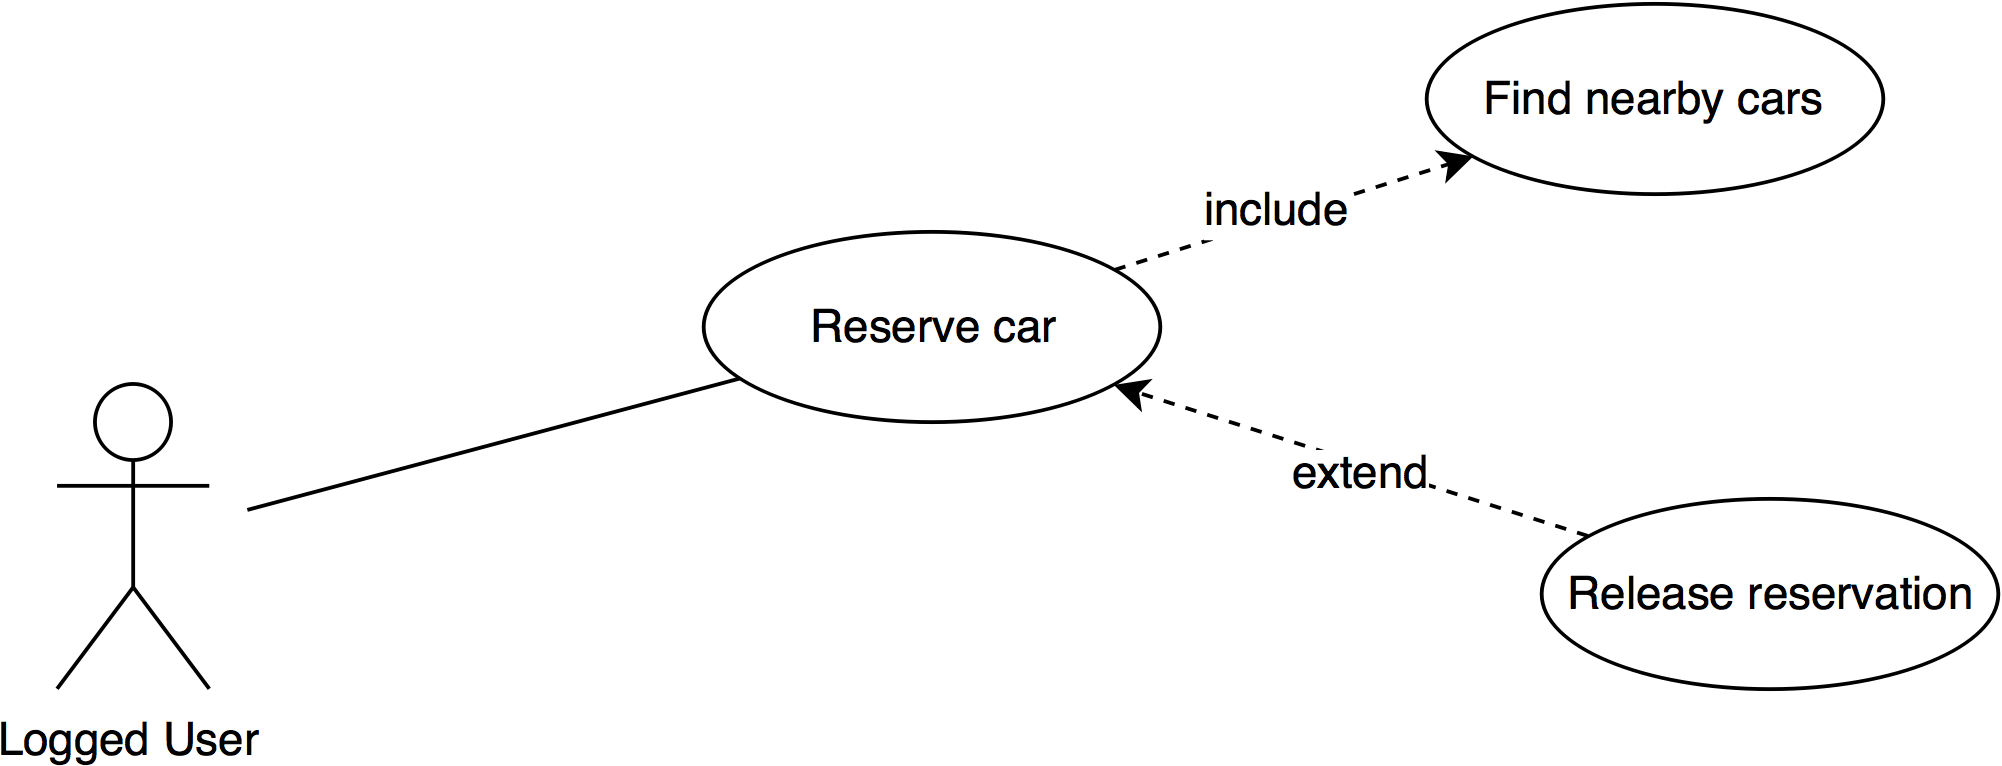
\includegraphics[width=\textwidth]{./specific_requirements/features/diagrams/request_car_uc.png}
		\caption{Extension of the use case diagram that includes the "Release reservation" feature}
		\label{request_car_uc}
\end{center}
\end{figure}

\begin{figure}[H]
\begin{center}
		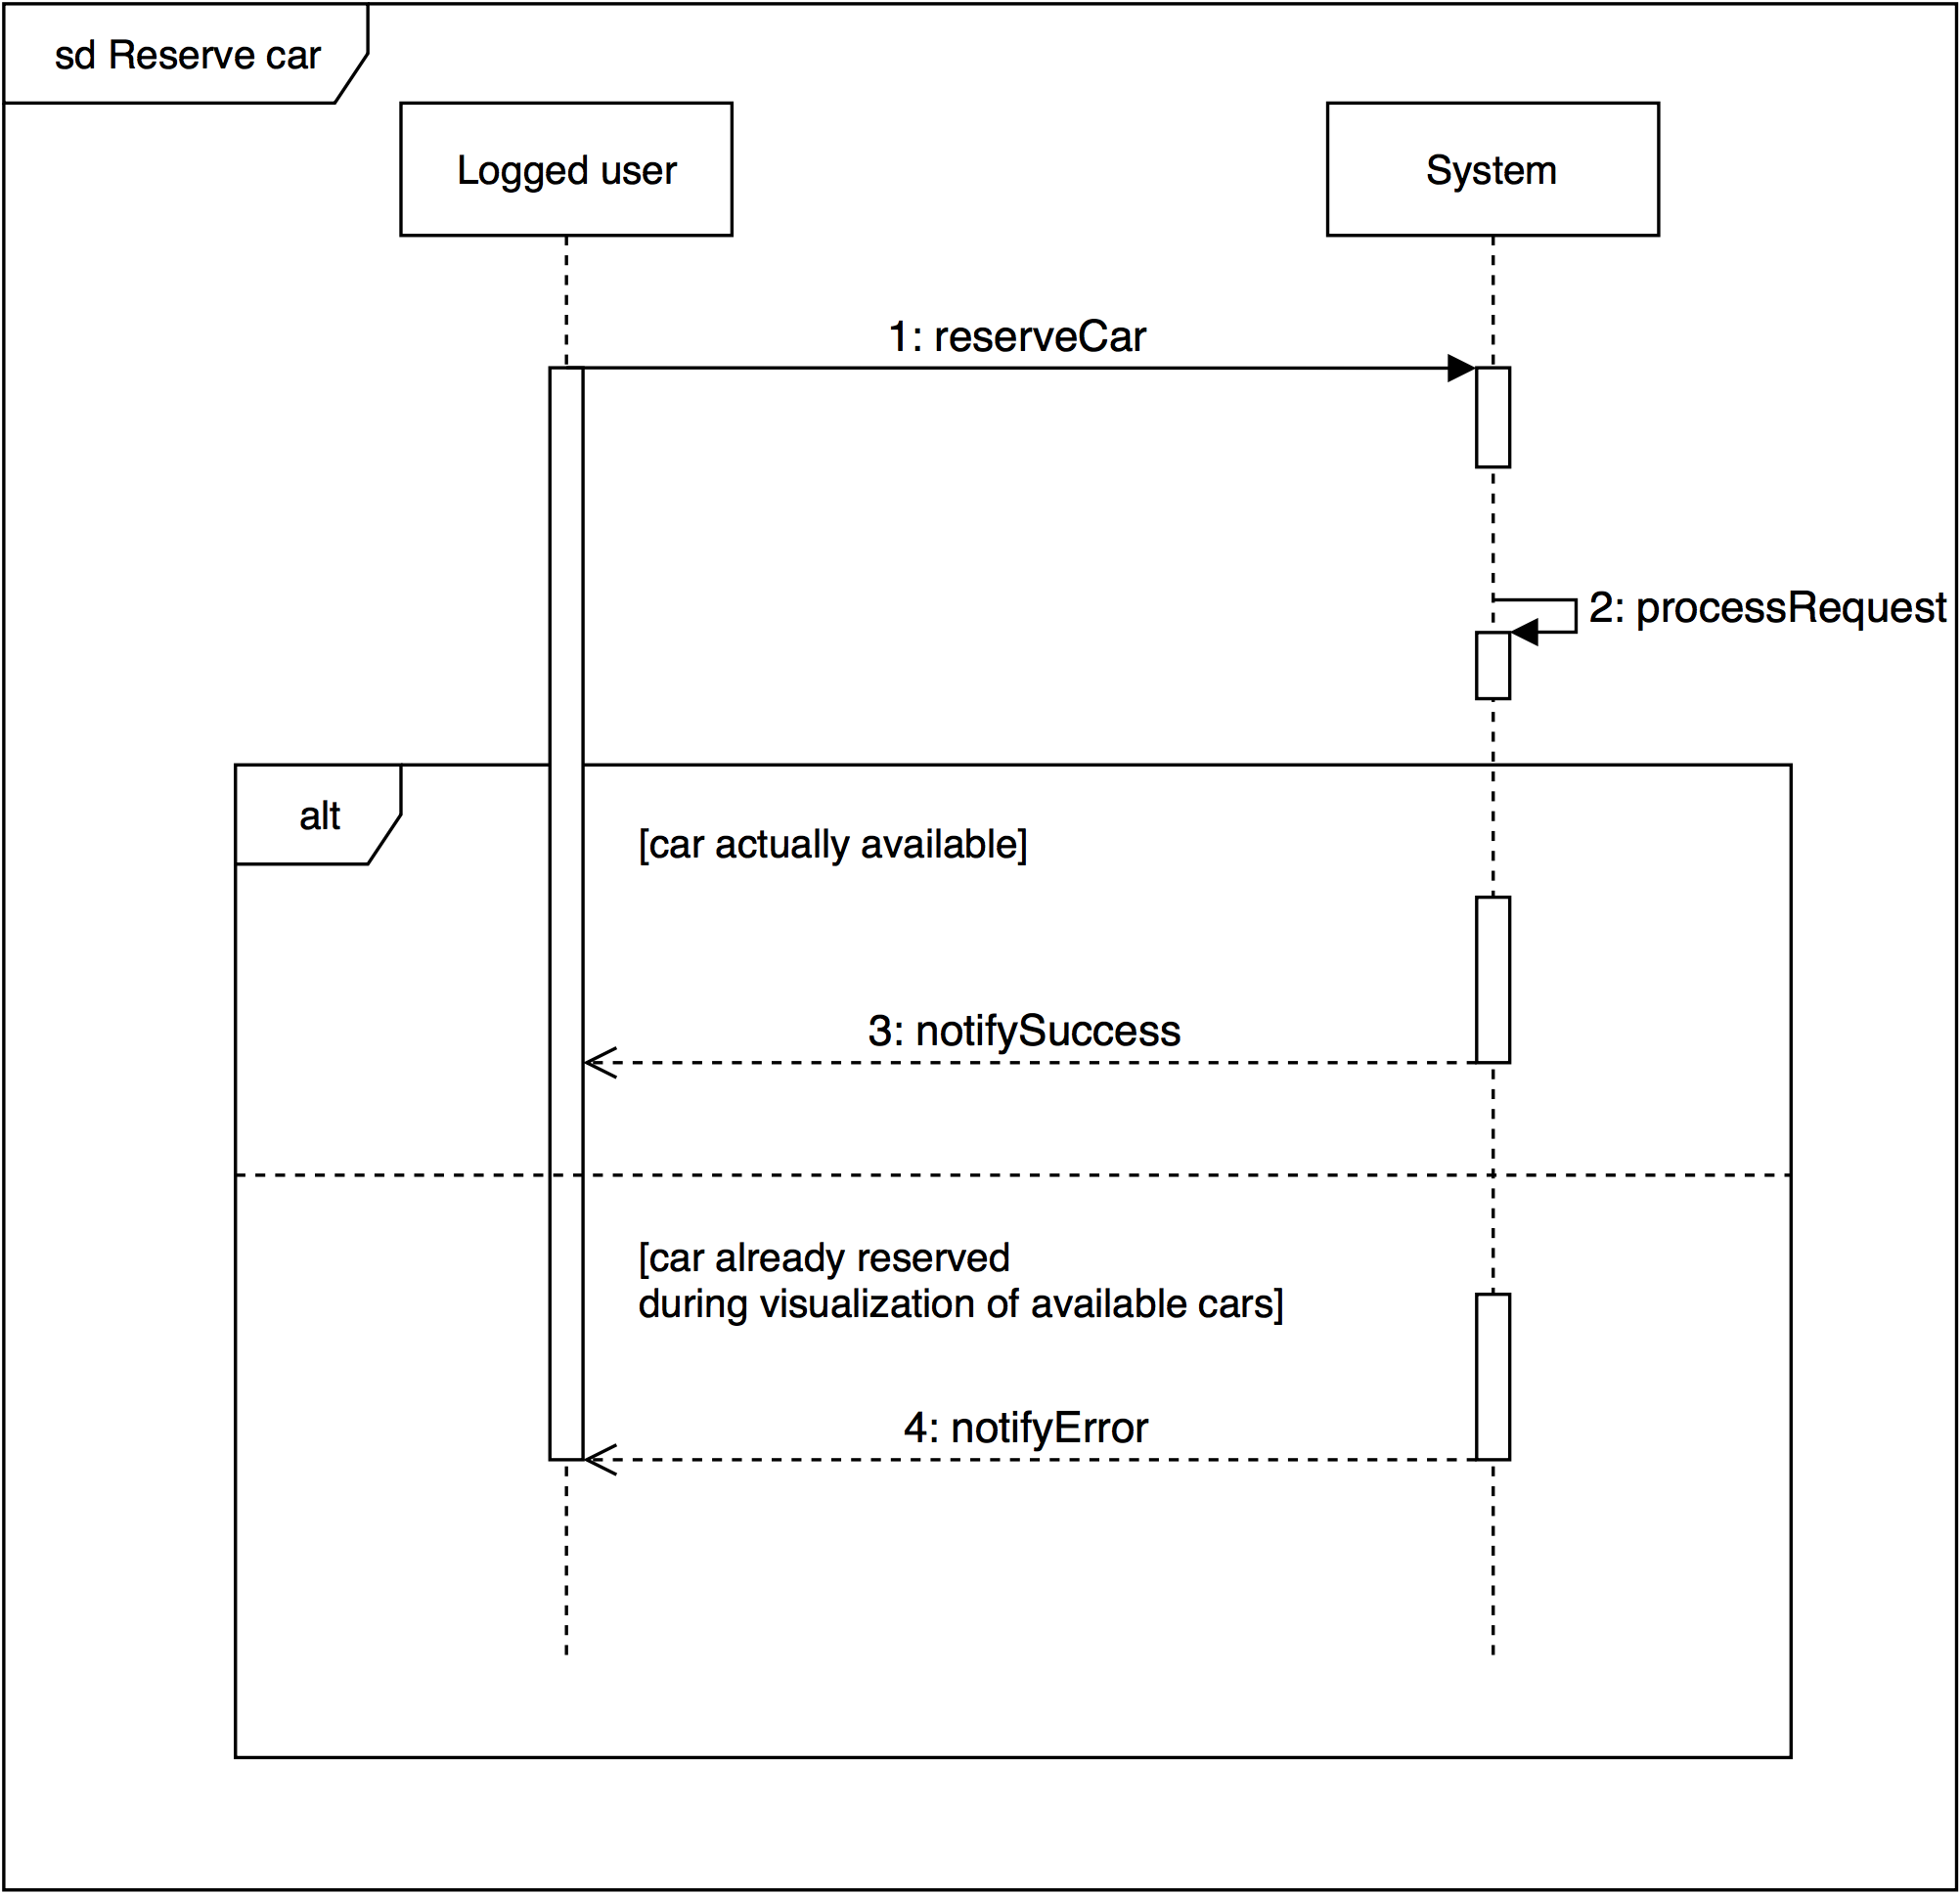
\includegraphics[width=\textwidth]{./specific_requirements/features/diagrams/reserve_car_sd.png}
		\caption{Sequence diagram that describes the event flow of a standard reservation request}
		\label{request_car_sd}
\end{center}
\end{figure}

\begin{table}[H]
\begin{center}
\begin{tabular}{p{0.3\textwidth} | p{0.7\textwidth}}
\hline
Actor & User\\
\hline
Goal & Goal 3\\
\hline
Input Condition & The user is logged in and has no active reservations\\
\hline
Event Flow & 
\begin{enumerate}
\item In the main page for the \emph{PowerEnJoy} website or mobile application, the user clicks or taps on the \emph{"Reserve car"} button;
\item The user inputs the desired location: specific address or current GPS location;
\item The system loads a map of the Safe Area, marking every available vehicle near the desired location;
\item The user clicks or taps on the car he/she wants to rent;
\item The user clicks or taps on the \emph{"Reserve this car"} button;
\item The system saves the registration in its database and logs it;
\item The system confirms the reservation to the user, reminding him/her of the fact that the reservation will expire in an hour of time with a small fee if the car is not actually used.
\end{enumerate} \\
\hline
Output Condition & The system notifies the user that the reservation was successful and marks the chosen car as reserved and not available.\\
\hline
Exception & If the user tries to reserve more than one car, the system notifies him/her that this action is forbidden. This happens when the following requirements are not satisfied: .

If the user changes his/her mind and decides not to reserve a car, the event flow stops at the point in which the map was shown. No car will be reserved in this eventuality.\\
\hline
\end{tabular}
\end{center}
\caption{Reserve car use-case}
\label{reserve_car_uc}
\end{table}

\begin{table}[H]
\begin{center}
\begin{tabular}{p{0.3\textwidth} | p{0.7\textwidth}}
\hline
Actor & User\\
\hline
Goal & Goal 3\\
\hline
Input Condition & The user is logged in and has an active reservation not older than an hour\\
\hline
Event Flow & 
\begin{enumerate}
\item In the main page for the \emph{PowerEnJoy} website or mobile application, the user clicks or taps on the \emph{"Reserve car"} button;
\item Since the user already reserved a car, he is shown the location and time of his current reservation;
\item The user clicks or taps on the \emph{"Release reservation"} button;
\item The system asks confirmation from the user;
\item The user confirms his/her choice of receding from his/her existing reservation;
\item The system modifies the state of the formerly reserved car marking it as available again and notifies the user of the fact that his/her reservation was successfully cancelled.
\end{enumerate} \\
\hline
Output Condition & The system notifies the user that the reservation was successfully cancelled and marks the chosen car as available again. The user can reserve another car, since he/she has no more active reservations\\
\hline
Exception & If the user changes his/her mind and wants to keep the current reservation, the event flow stops at the point in which the current reservation was shown. The reservation will be kept unchanged in this eventuality.\\
\hline
\end{tabular}
\end{center}
\caption{Reserve car use-case for the option of releasing a reservation}
\label{reserve_car_uc_alt}
\end{table}

\begin{figure}[H]
\begin{center}
		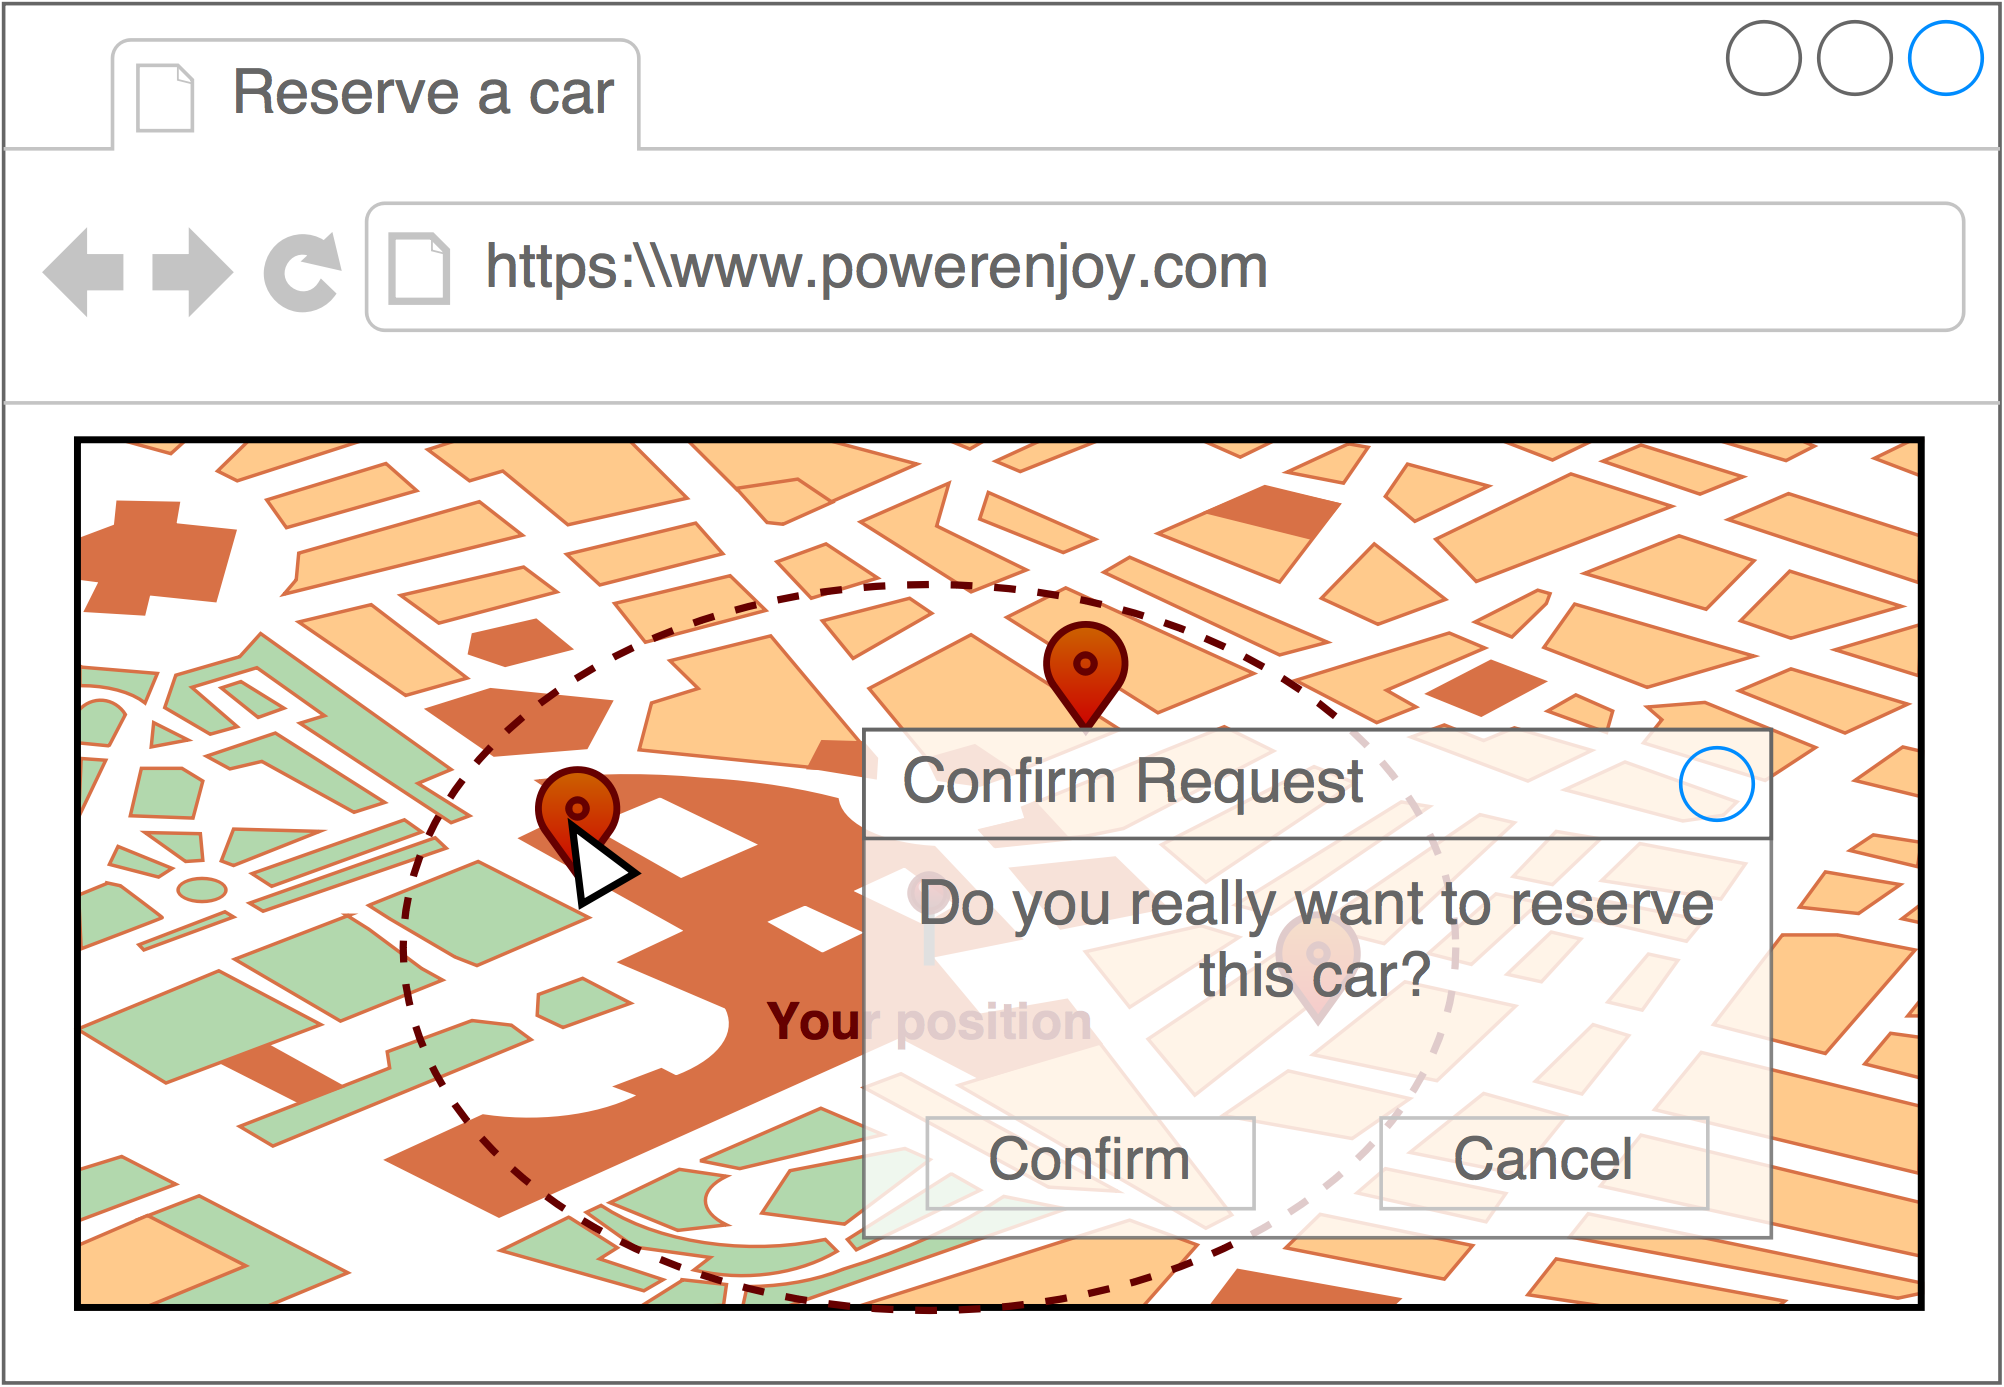
\includegraphics[width=\textwidth]{./specific_requirements/features/diagrams/web_reserve_car.png}
		\caption{Mockup of the reservation web page}
		\label{web_reserve_car}
\end{center}
\end{figure}

\subsection{Use Car}
\subsubsection{Purpose}
The use car feature is the key feature of the whole system. For the sake of completeness, this requirement is described by detailing each of its sub-parts, as seen in Figure \ref{global_uc}.
The detailed sub-parts are described in the subsections immediately after this one, namely: \ref{unlock_car_section}.

Its purpose is that of allowing users to open, get on and drive the actual vehicle that they rented via the dedicated service. This feature requires the interaction of the user with both his/her mobile device and the on-board computer application.

The system must unlock a car upon being provided with the PIN from the user that reserved it. The on-board computer application must keep track of every important detail of user rides, such as the current charges, the nearby free charging spots and the boundaries of the Safe Area, all while notifying correspondingly the driver.

The on-board computer application will detect the beginning and end of the ride, counting the charges accordingly. Also, the system will be able to detect wheter the car is inside the Safe Area or not: if this is not the case, the user will be notified and the charges will keep increasing.

\subsection{Unlock Car} \label{unlock_car_section}
\subsubsection{Purpose}
This sub-part of the "Use Car" functionality focuses on the sequence of sub-functionalities involved in the car unlocking process.

The purpose of the functionality is that of allowing the user to unlock the car he/she reserved based on his/her actual proximity to the vehicle - given the GPS of a mobile device is available - or upon the insertion of a vehicle-specific code into the application.

\subsubsection{Scenario 1}
Damian reserved a \emph{PowerEnJoy} car and is walking towards the vehicle location. When he reaches the car, he takes out his smartphone and opens the \emph{"Reserve Car"} function of the mobile app. The system shows the current reservation: since Damian is close enough to the car and the GPS is active on his mobile device, the \emph{"Unlock car"} button has been activated. He taps on the button and the car unlocks, enabling him to enter it.

\subsubsection{Scenario 2}
Elsa stayed out later than usual to study for her exams, and decided to rent a \emph{PowerEnJoy} car with her laptop. Her smartphone has low battery, so she decided to turn the GPS off to make the battery last longer. Once she gets to the car, she tries to unlock it by making the system detect her proximity. Since the button does not activate, she remembers that the GPS is off and decides to input the car code into the mobile app; she then finds the dedicated car code, opens the right function by tapping on the \emph{"Unlock with car code"} button and inputs it. The system processes the request and, having verified that the user who inserted the code is the same who reserved the car, properly unlocks the vehicle and lets Elsa enter it.

\subsubsection{Use-case}
A detail of the use-case is provided in Table \ref{unlock_car_uc}

\subsubsection{Functional requirements}
\begin{enumerate}
\item Upon every try, the system must check that the user trying to unlock the car is the same that reserved it;
\item The system must guarantee to recognize the proximity of the user if he/she is within a 2 m radius from the car and has the GPS active on a mobile device;
\item The system must always guarantee the possibility for the user to unlock the vehicle he/she reserved by inserting the car code instead of using the GPS proximity detection system;
\item Upon every code insertion, the system must check that the code is the one associated with the car reserved by the user who inserted the code;
\item The vehicle-specific code must be unique for each car.
\item The reservation expiration timer must stop as soon as the car is unlocked;
\end{enumerate}

\begin{table}[H]
\begin{center}
\begin{tabular}{p{0.3\textwidth} | p{0.7\textwidth}}
\hline
Actor & Logged user\\
\hline
Goal & Goal 5\\
\hline
Input Condition & The user reserved a car and is in its proximity OR The user reserved a car inserted the car code into the application\\
\hline
Event Flow & 
\begin{enumerate}
\item The user who reserved the vehicle approaches it and opens the mobile application;
\item The user opens the \emph{"Reserve car"} function and the system provides the sum-up of his/her active reservation;
\item The user either: has the GPS active and taps onto the \emph{"Unlock car"} button OR reads and inserts the car code into the application, tapping the \emph{"Unlock with car code"} button;
\item The system processes the request, by verifying that the user who tries to unlock the car is the one who reserved it;
\item The system unlocks the vehicle.
\end{enumerate} \\
\hline
Output Condition & The car is unlocked and the user can access it.\\
\hline
Exception & If the user wants to unlock the car but he/she is further than 2 m away from it, the \emph{"Unlock car"} button on the reservation screen will not be active.

If the user inputs a wrong code when trying to unlock the car, the system will notify that the code is wrong and will not unlock the car, sending the user back to the reservation page on the application.\\
\hline
\end{tabular}
\end{center}
\caption{Unlock car use-case}
\label{unlock_car_uc}
\end{table}

\begin{figure}[H]
\begin{center}
		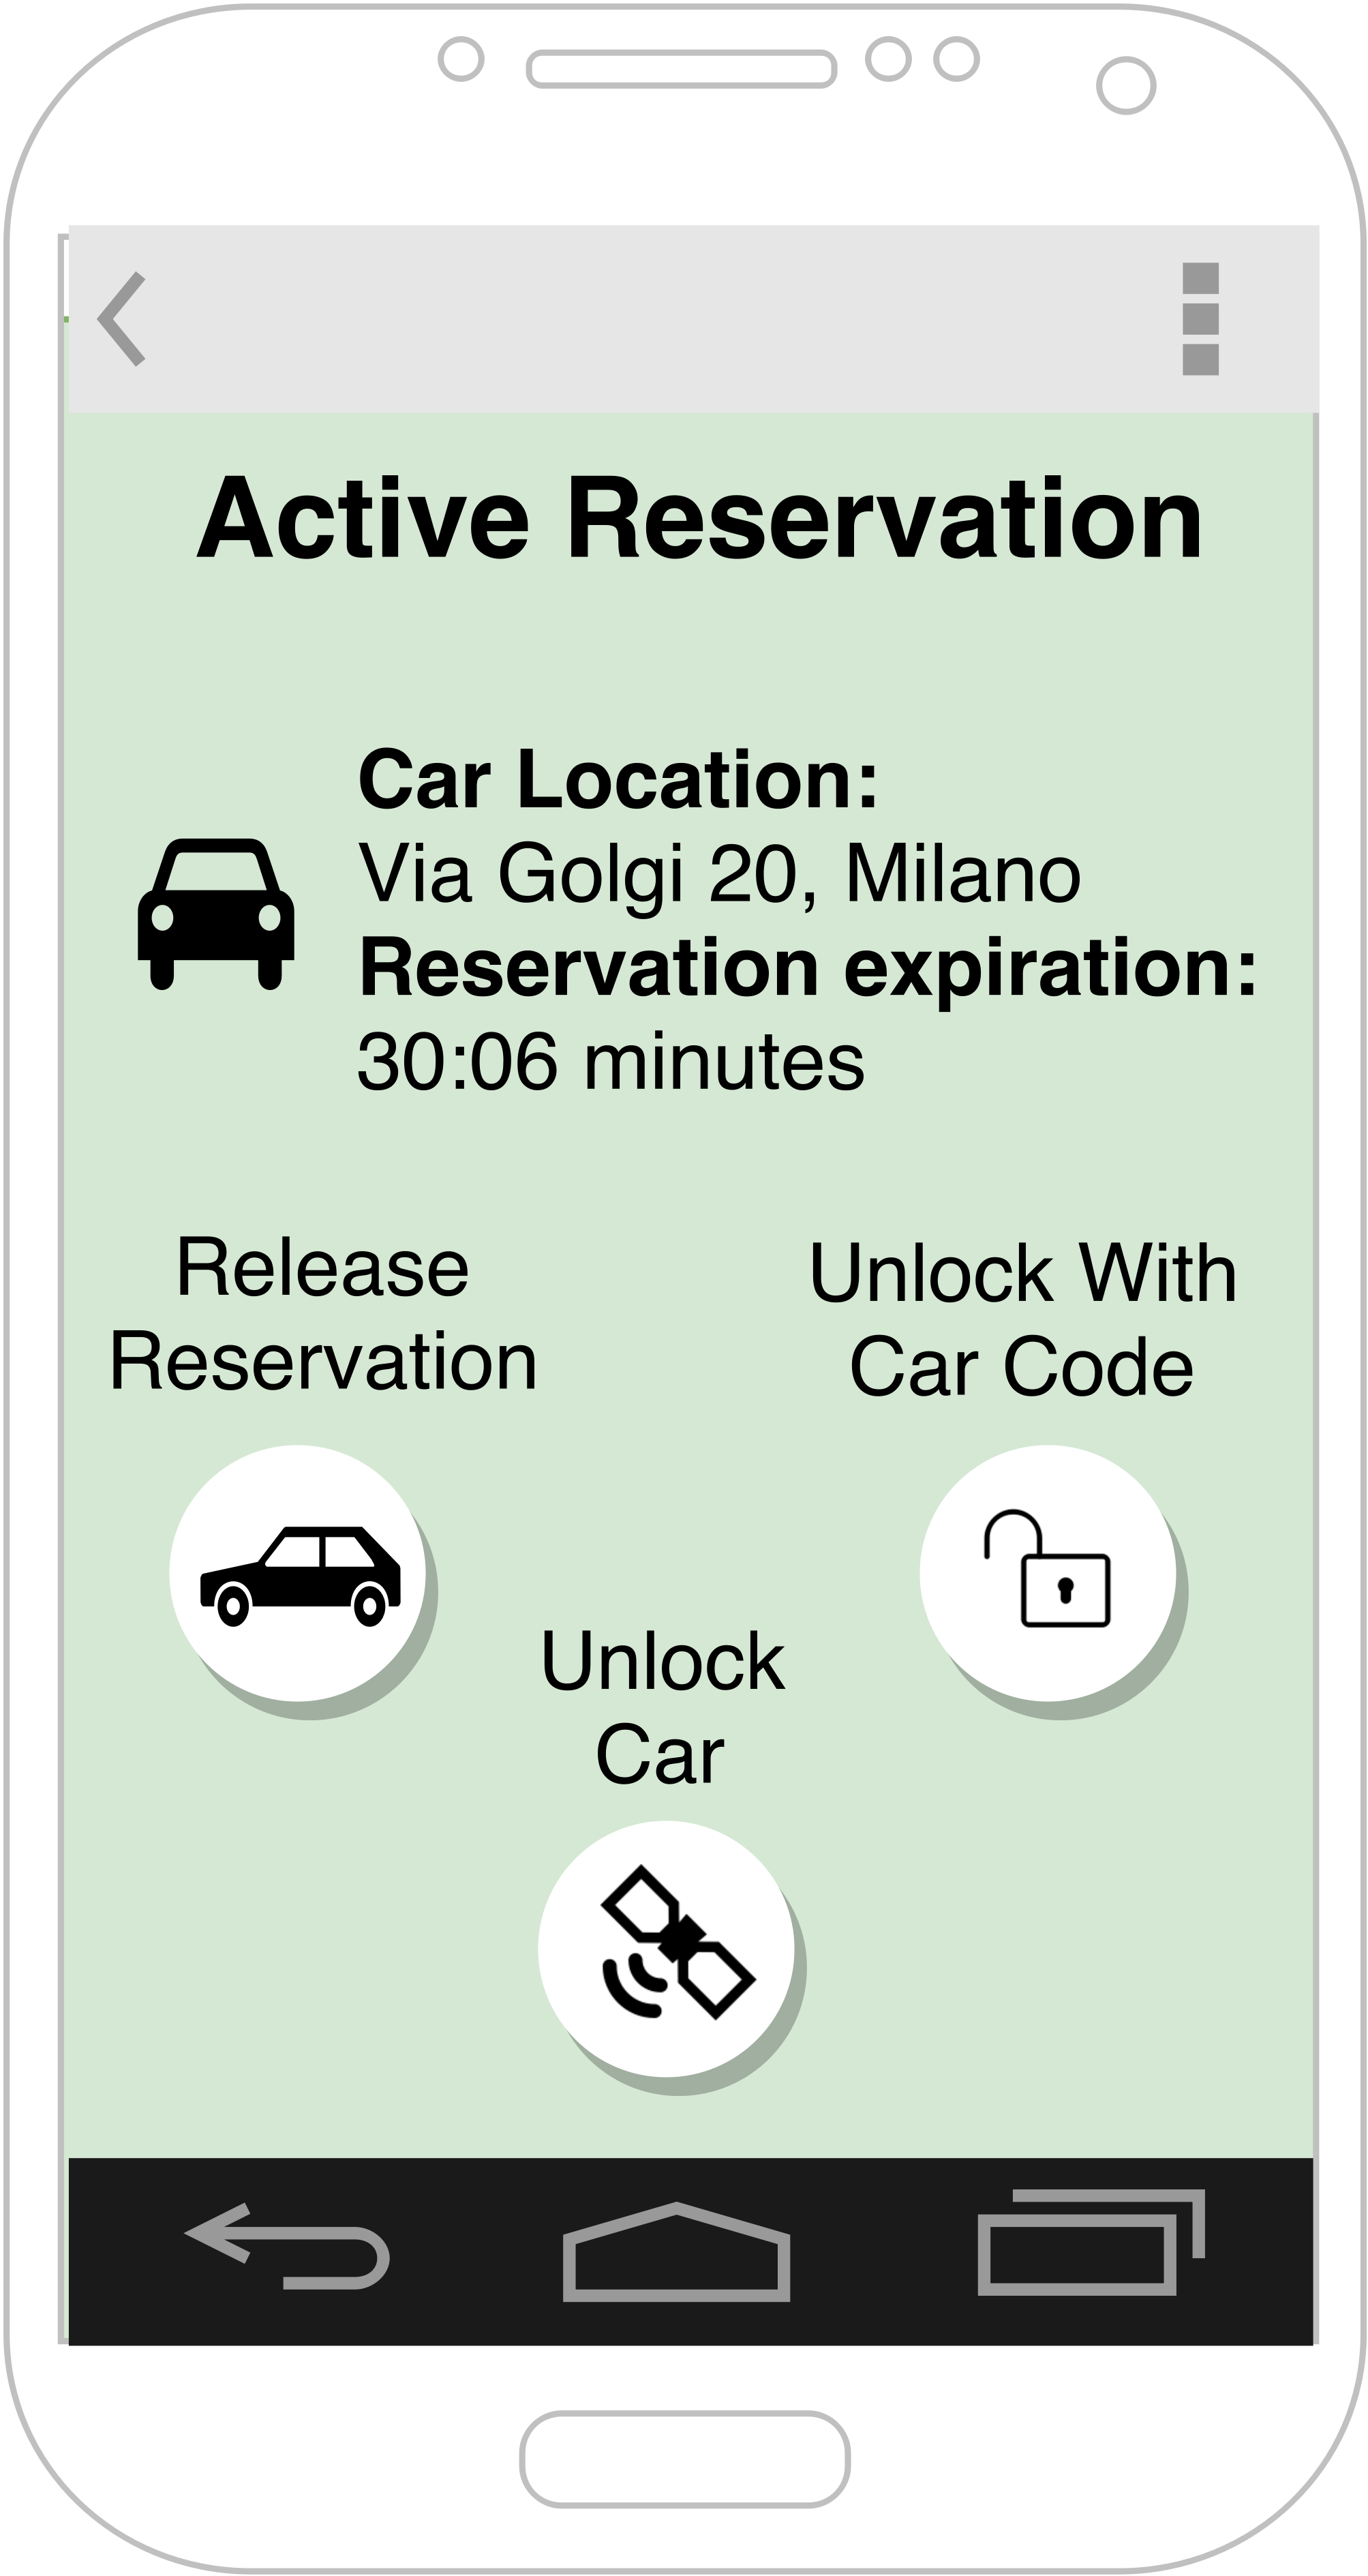
\includegraphics[width=0.4\textwidth]{./specific_requirements/features/diagrams/mobile_unlock.png}
		\caption{Mockup of the mobile unlock feature accessible from the reservation screen.}
		\label{mobile_unlock}
\end{center}
\end{figure}

\subsection{Start Ride} \label{start_ride_section}
\subsubsection{Purpose}
This sub-part of the "Use Car" functionality focuses on the sub-functionalities concerned with the interaction between the user and the on-board application in order to allow the user to turn the engine on.

The system will interact with the user prompting him/her after the car has been unlocked and asking to proceed with the specified authentication method. This process will grant access to the car systems, hence allowing the user to start the ride and igniting the engine.

The on-board application will also start charging the user as soon as he/she authenticates, all while showing him/her the current charges on the screen, along with the sat-nav that is also going to signal nearby charging stations and the boundaries of the Safe Area.

\subsubsection{Scenario 1}
Francis just unlocked the car he reserved using the \emph{PowerEnJoy} service. He sits on the driver's side and closes the door. The screen of the on-board computer is turned on and the system prompts Francis to authenticate. He performs the authentication procedure correctly; the message \emph{"You can now turn the engine on. The system is charging you based on the duration of the ride."} appears on the screen. Francis turns the engine on and he then proceeds to drive the car, starting his ride.

\subsubsection{Scenario 2}
Graham mounted on a \emph{PowerEnJoy} vehicle he just reserved and unlocked. When he authenticates after being prompted by the system, he makes an error. The system then shows an error message. Graham then repeats the procedure properly; this time it is correct, and the system allows him to drive the car.

\subsubsection{Use-case}
A detail of the use-case is provided in Table \ref{start_ride_uc}.

\subsubsection{Sequence diagram}
A UML sequence diagram is provided to detail the standard behavior of the system upon performance of the authentication method. The diagram is in Figure \ref{start_sd}.

\subsubsection{Functional Requirements}
\begin{enumerate}
\item The system must check that the authentication method is followed properly;
\item The system must start charging the user only after he/she authenticates;
\item The system must always notify the user about his/her current charges;
\item The system must mark the car as "in-use" as soon as the user authenticates;
\end{enumerate}

\begin{figure}[H]
\begin{center}
		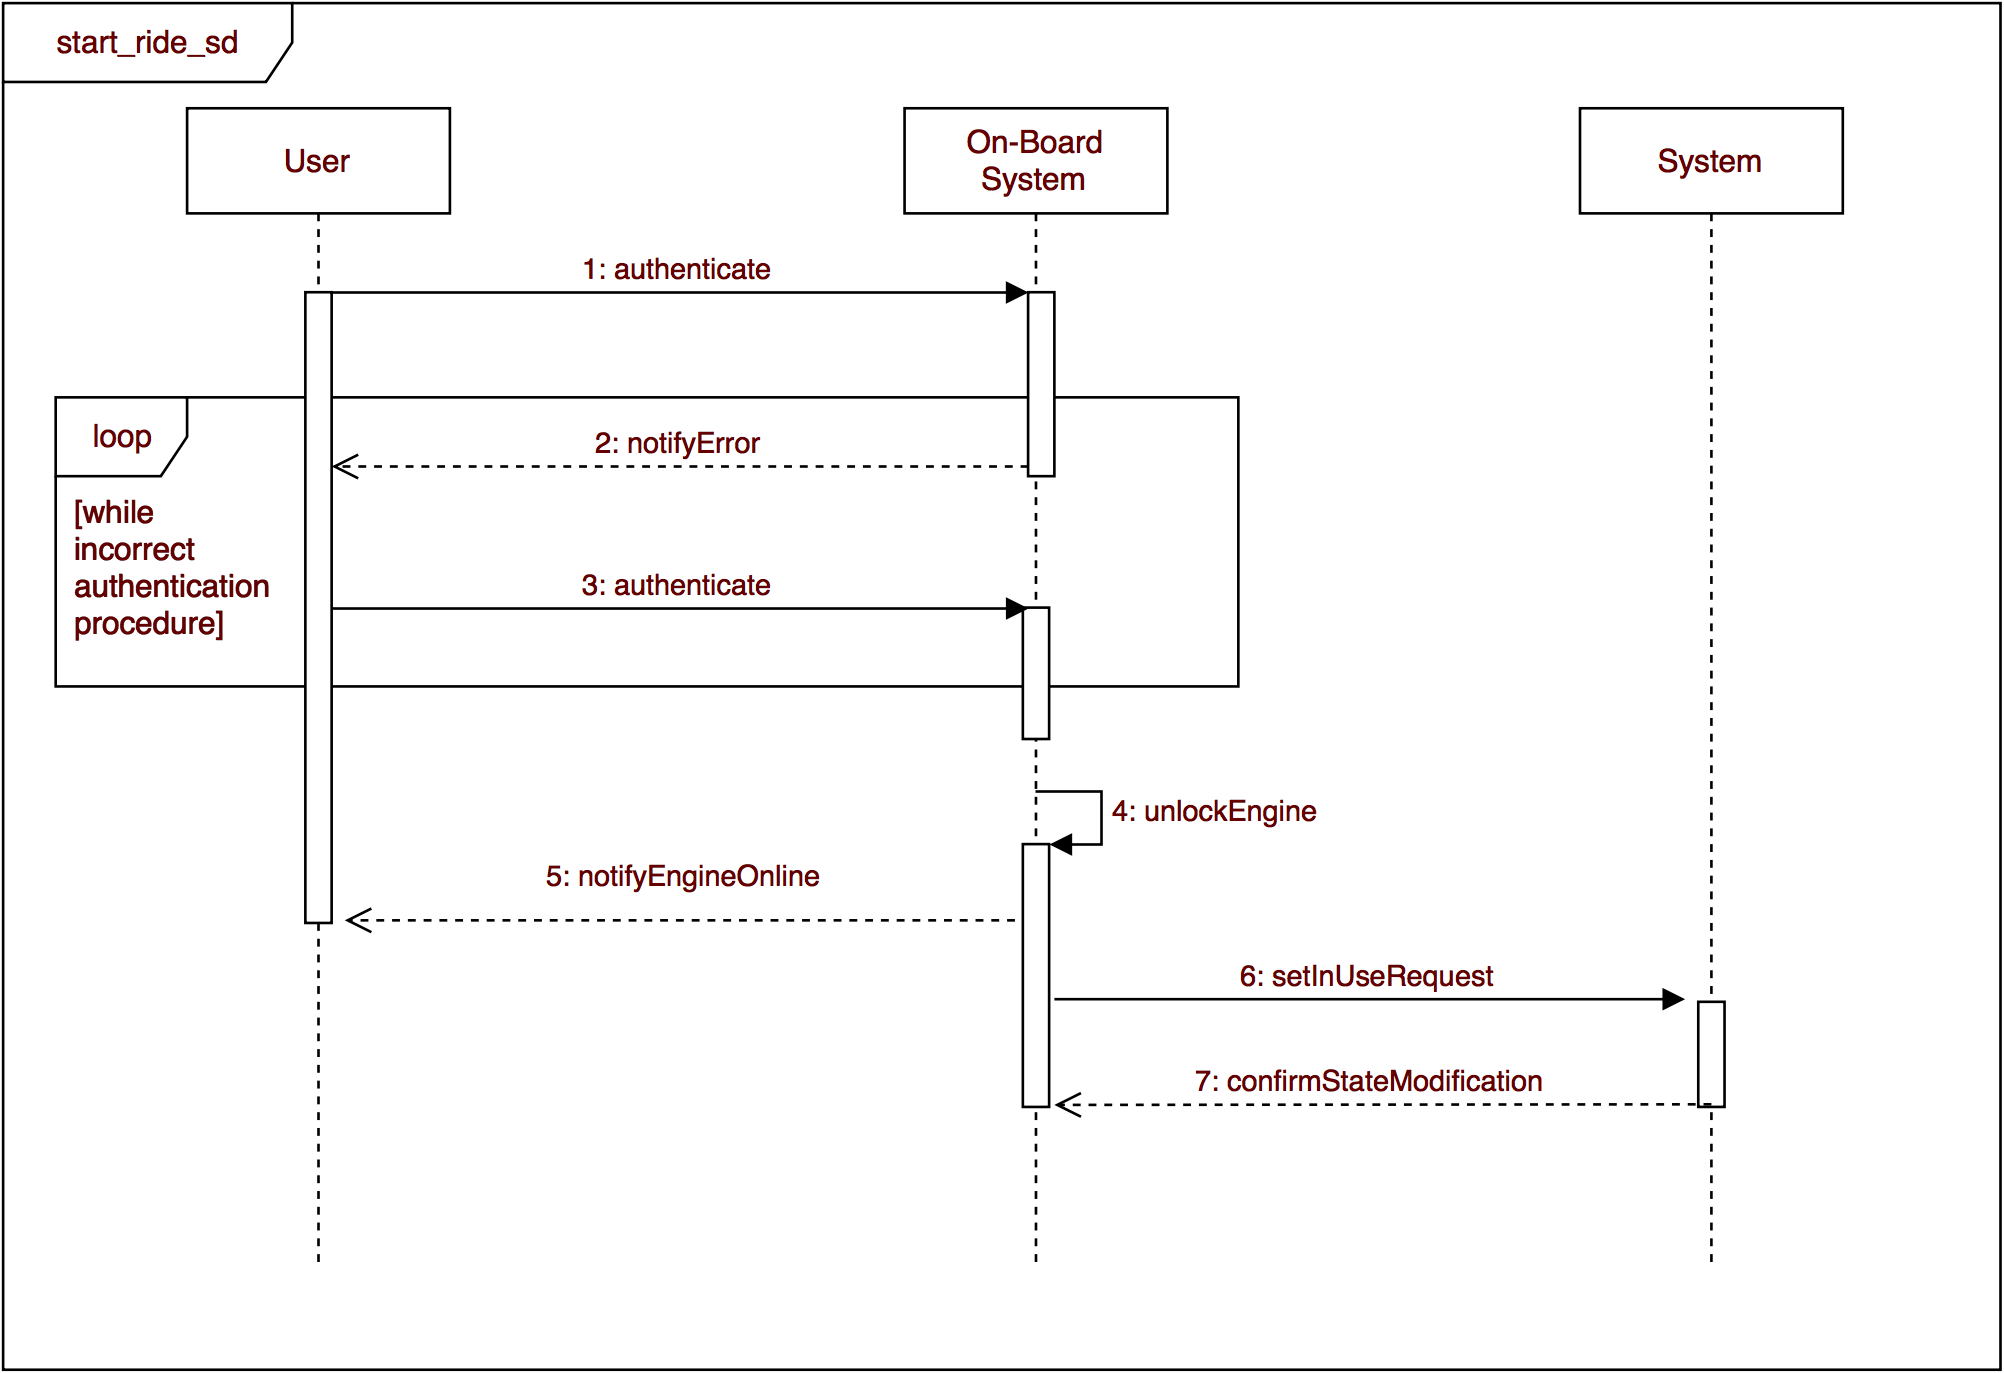
\includegraphics[width=\textwidth]{./specific_requirements/features/diagrams/start_ride_sd.png}
		\caption{Sequence diagram for the process of starting a ride in a standard situation.}
		\label{start_sd}
\end{center}
\end{figure}

\begin{table}[H]
\begin{center}
\begin{tabular}{p{0.3\textwidth} | p{0.7\textwidth}}
\hline
Actor & User\\
\hline
Goal & Goal 7\\
\hline
Input Condition & The user unlocked the car.\\
\hline
Event Flow & 
\begin{enumerate}
\item The user performs the authentication procedure interacting with the on-board screen;
\item The system analyzes the procedure correctness;
\item The system starts charging the user and marks the car as "in-use";
\item The system lets the user to turn on the engine.
\end{enumerate} \\
\hline
Output Condition & The user ignites the engine and starts the ride.\\
\hline
Exception & If the user makes an error while authenticating, the system will notify it and report an error message; in this case, the car still can not be turned on and its status remained "Reserved".\\
\hline
\end{tabular}
\end{center}
\caption{Start ride use-case}
\label{start_ride_uc}
\end{table}

\subsection{Pay Fee}
\subsubsection{Purpose}
The system must prevent any user's unfair behavior. Whenever the user decides to reserve a car for a ride, he/she has a limited amount of time to reach the car and use it. This is reasonable because during this time nobody can rent that precise car. If the user does not come and use the reserved car, he/she must be penalized and fined by the system.

Moreover, in this case, the previously reserved car becomes available again and the system notify the bad user about the fine he/she has just received. Then the system talks to the payment handler which automatically charges the user.

\subsubsection{Scenario 1}
Negan is dancing at the disco with his friends when he realizes that it's very late. He opens the \emph{PowerEnJoy} application on his smartphone and checks for an available and nearby car to rent to go home. He finds one and reserve it.

Suddenly he notices a very beautiful girl and decides to speak to her in order to know her better. The clock is ticking and he forgets about his previous reservation. After more than one hour, Negan checks his mobile phone and notices the system has notified him about the expired reservation charging a fine.

\subsubsection{Use-case}
The pay fee use-case is shown in Table \ref{pay_fee_uc}.

\subsubsection{Functional requirements}
\begin{enumerate}
\item The system must not allow a car to be reserved for more than 1 hour;
\item The system must notify the user about the expired reservation;
\item The system automatically charges the user in case of reservation expiration;
\item If the reserved car is not picked-up by the user within 1 hour from the reservation, the system tags the car available again;
\end{enumerate}

\begin{table}[H]
\begin{center}
\begin{tabular}{p{0.3\textwidth} | p{0.7\textwidth}}
\hline
Actor & Bad user, payment handler\\
\hline
Goal & Goal 4\\
\hline
Input Condition & The user has reserved a car and he/she does not pick it up within 1 hour from the reservation\\
\hline
Event Flow & 
\begin{enumerate}
\item The system establish a connection to the payment handler;
\item The system asks the payment handler to charge the user a fee of 1 euro;
\end{enumerate} \\
\hline
Output Condition & The system notifies the user about the fine and tags the reserved car available again.\\
\hline
%Inserire errore nel pagamento?
Exception & None.\\
\hline
\end{tabular}
\end{center}
\caption{Pay fee use-case}
\label{pay_fee_uc}
\end{table}

\section{Performance Requirements} \label{per_req}
The following performance requirements must be satisfied by the system-to-be in order to guarantee the best user experience:
\begin{itemize}
\item The system must not have an upper-bound as far as the total number of registered users is concerned;
\item The system must handle at least 1000 active reservations at the same time;
\item The system must simultaneously support at least 1000 logged users who want to take the advantage of the service performing any kind of operation;
\item 90\% of car unlock requests shall be processed in less than 1 s;
\item 100\% of car unlock requests shall be processed in less than 2 s;
\item 100\% of any other kind of requests shall be processed in less than 5 s.

Since the performance is essentially bound by the internet connection, the above timing constraints are to be intended from when the system receives the request to the dispatch of the reply.
\end{itemize}

\section{Software System Attributes} \label{software_sys_attr}
\subsubsection{Reliability}
The reliability of the system depends on several factors. First of all it is related to the reliability of the servers that run the back-end application. In addition to that, the reliability of the on-board computers must be also taken into account. Therefore the probability of failure of the devices mentioned above heavily affects the overall system reliability, that can be evaluated as:
\begin{center}
	\[\emph{Reliability} = 1-\emph{Probability of failure}\]
\end{center}

\subsubsection{Availability}
The system must offer an availability of 99\%. The remaining 1\% shall take into account the time spent for ordinary maintenance sessions.

\subsubsection{Security}
\begin{itemize}
\item All the connections established between users and server must use the HTTPS protocol;
\item All the communications between the server and the payment handler shall be encrypted;
\item The users' passwords are stored in the database using a proper hashing mechanism;
\item The system keeps track of all the login attempts storing the corresponding IP addresses.
\end{itemize}

\subsubsection{Maintainability}
The code of the whole software-to-be-developed must be thoroughly documented in order to let future developers easily know how the system works and how it has been designed. A version control system must be used to manage and organize all the different code revisions.

\subsubsection{Portability}
The server-side of the application shall be written in Java. Therefore it can be executed on any platform that supports the Java Virtual Machine and runs JEE. The web application must support the latest version of the main browsers like IE, Google Chrome and Firefox. The mobile application must be developed for both Android and iOS architectures.
The car-side of the application is designed to run on the existing on-board computers.


\section{Alloy} \label{alloy}
This section includes a class diagram which is representative of the relevant features of the system-to-be, followed by the Alloy code that describes and checks the consistency of the model provided in this document, as well as an example of the model-compliant world generated by the Alloy tool.

\begin{figure}[H]
\begin{center}
		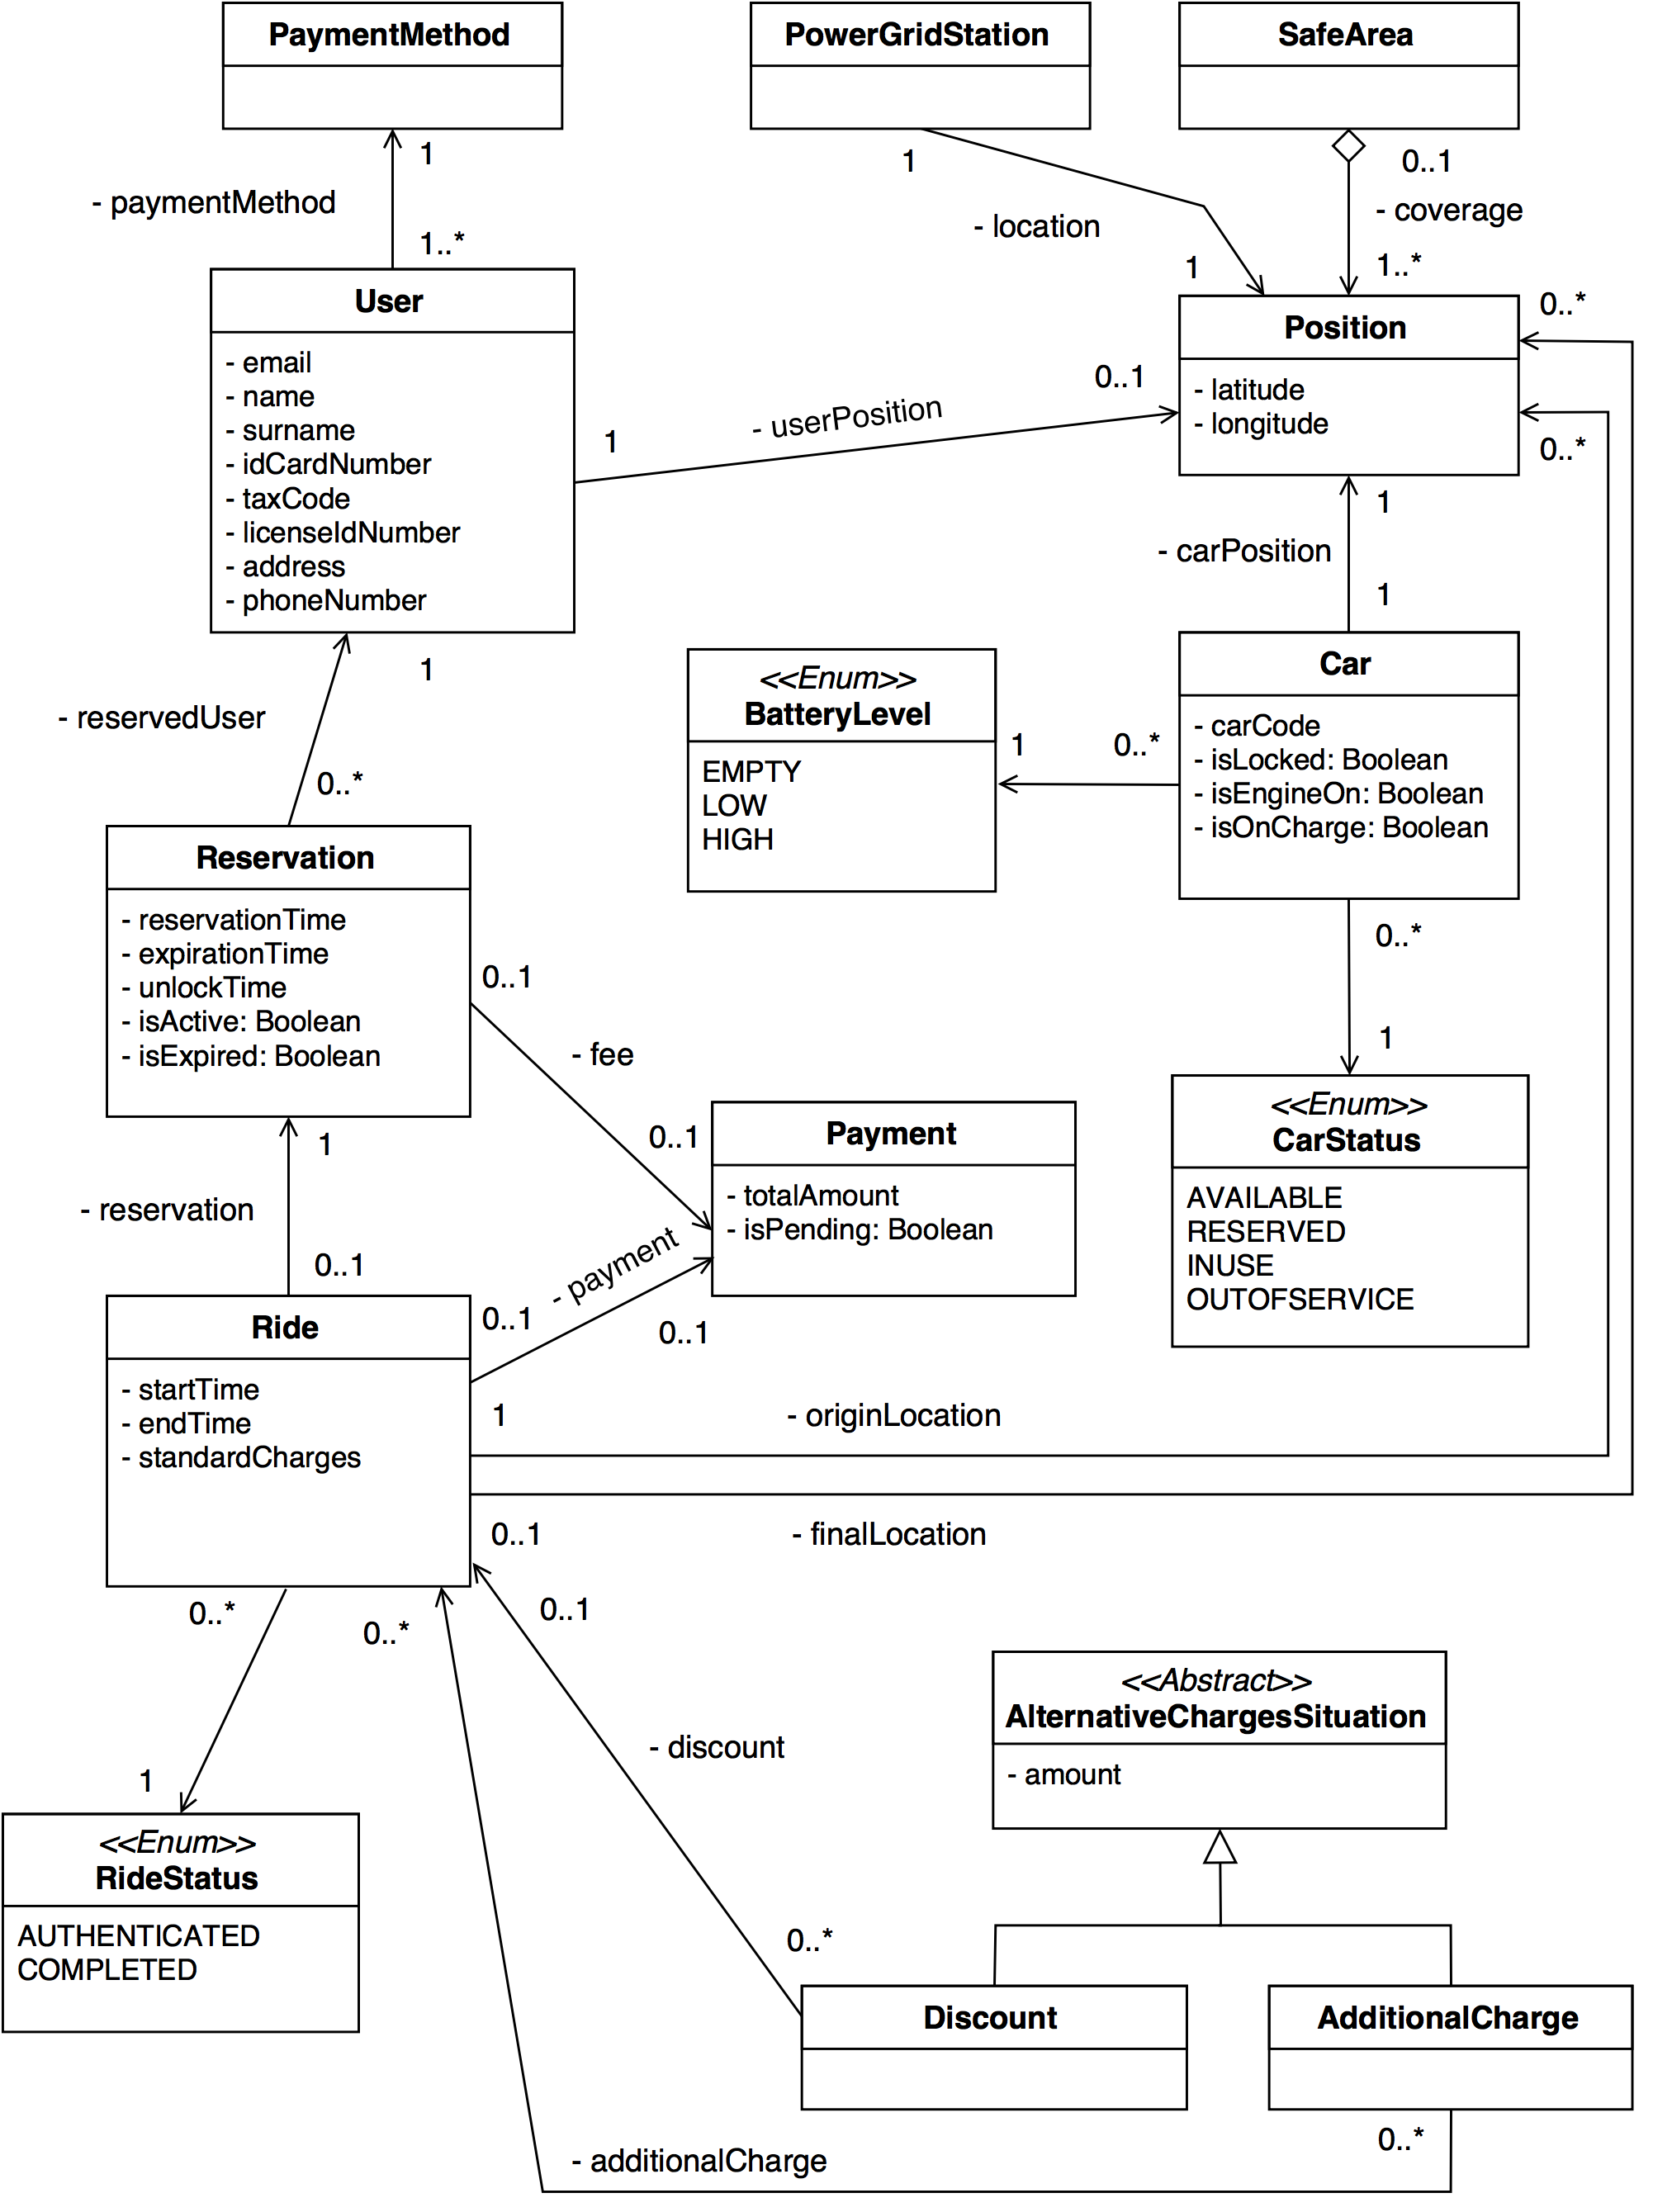
\includegraphics[width=\textwidth]{./pictures/class_diagram.png}
		\caption{Class diagram illustrating the structure of the system-to-be.}
		\label{class_diagram}
\end{center}
\end{figure}

% Settings for Alloy code listing.
\lstset{
    language=alloy,
    numbers=left,
    numberstyle=\tiny,
    stepnumber=2,
    tabsize=4,
    keywordstyle=\color{alloy-keyword}\bfseries,
    commentstyle=\color{alloy-comment},
    stringstyle=\color{alloy-string},
    basicstyle=\small\fontfamily{pcr}\selectfont, % Courier font family
}

% Includes the Alloy model file.
\lstinputlisting{./specific_requirements/alloy/alloy_pe.als}


\appendix
\chapter{Appendix}
\section{Software and tools used}
\begin{itemize}
\item \LaTeX, used as typesetting system to build this document.
\item draw.io - \url{https://www.draw.io} - used to draw diagrams and mock-ups.
\item GitHub - \url{https://github.com} - used to manage the different versions of the document and to make the distributed work much easier.
\item GitHub Desktop, the GitHub official application that offers a seamless way to contribute to projects.
\end{itemize}
\section{Hours of work}
The absolute major part of the document was produced in group work. The approximate number of hours of work for each member of the group is the following:

\begin{itemize}
\item Giovanni Scotti: 25 hours
\item Marco Trabucchi: 20 hours
\end{itemize}

NOTE: indicated hours include the time spent in group work.

\begin{thebibliography}{1}

\bibitem{ieee-29148}
	ISO/IEC/IEEE 29148:2011 \emph{Systems and software engineering - Life cycle processes - Requirements engineering}
	
\bibitem{se-assignments}
	AA 2016/2017 Software Engineering 2 - \emph{Project goal, schedule and rules}

\end{thebibliography}

\end{document}